% !TeX encoding = UTF-8
% !TeX program = xelatex
% !TeX spellcheck = en_US

\documentclass[degree=bachelor]{thuthesis}
\usepackage{listings}
\usepackage{xcolor}
\renewcommand{\lstlistingname}{清单}

\lstset{
    basicstyle=\ttfamily\small,
    commentstyle=\color{gray},
    keywordstyle=\color{blue},
    stringstyle=\color{red},
    breaklines=true,
    frame=single,
    numbers=none,
    numberstyle=\tiny\color{gray},
    captionpos=b
}

  % 学位 degree:
  %   doctor | master | bachelor | postdoc
  % 学位类型 degree-type:
  %   academic(默认)| professional
  % 语言 language
  %   chinese(默认)| english
  % 字体库 fontset
  %   windows | mac | fandol | ubuntu
  % 建议终版使用 Windows 平台的字体编译


% 论文基本配置,加载宏包等全局配置
% !TeX root = ./thuthesis-example.tex

% 论文基本信息配置

\thusetup{
  %******************************
  % 注意:
  %   1. 配置里面不要出现空行
  %   2. 不需要的配置信息可以删除
  %   3. 建议先阅读文档中所有关于选项的说明
  %******************************
  %
  % 输出格式
  %   选择打印版(print)或用于提交的电子版(electronic),前者会插入空白页以便直接双面打印
  %
  output = print,
  % 格式类型
  %   默认为论文(thesis),也可以设置为开题报告(proposal)
  % thesis-type = proposal,
  %
  % 标题
  %   可使用“\\”命令手动控制换行
  %
  title  = {操作系统宏内核内存管理模块的设计与实现},
  title* = {Design and Implementation of the Macro Kernel Memory Management Module in Operating System},
  %
  % 学科门类
  %   1. 学术型
  %      - 中文
  %        需注明所属的学科门类,例如:
  %        哲学、经济学、法学、教育学、文学、历史学、理学、工学、农学、医学、
  %        军事学、管理学、艺术学
  %      - 英文
  %        博士:Doctor of Philosophy
  %        硕士:
  %          哲学、文学、历史学、法学、教育学、艺术学门类,公共管理学科
  %          填写“Master of Arts“,其它填写“Master of Science”
  %   2. 专业型
  %      直接填写专业学位的名称,例如:
  %      教育博士、工程硕士等
  %      Doctor of Education, Master of Engineering
  %   3. 本科生不需要填写
  %
  % degree-category  = {工学硕士},
  % degree-category* = {Master of Science},
  %
  % 培养单位
  %   填写所属院系的全名
  %
  department = {计算机科学与技术系},
  %
  % 学科
  %   1. 研究生学术型学位,获得一级学科授权的学科填写一级学科名称,其他填写二级学科名称
  %   2. 本科生填写专业名称,第二学位论文需标注“(第二学位)”
  %
  discipline  = {计算机科学与技术},
  discipline* = {Computer Science and Technology},
  %
  % 专业领域
  %   1. 设置专业领域的专业学位类别,填写相应专业领域名称
  %   2. 2019 级及之前工程硕士学位论文,在 `engineering-field` 填写相应工程领域名称
  %   3. 其他专业学位类别的学位论文无需此信息
  %
  % professional-field  = {计算机技术},
  % professional-field* = {Computer Technology},
  %
  % 姓名
  %
  author  = {陈羿华},
  author* = {Chen Yihua},
  %
  % 学号
  % 仅当书写开题报告时需要(同时设置 `thesis-type = proposal')
  %
  % student-id = {2000310000},
  %
  % 指导教师
  %   中文姓名和职称之间以英文逗号“,”分开,下同
  %
  supervisor  = {陈渝, 副教授},
  supervisor* = {Associate Professor Chen Yu},
  %
  % 副指导教师
  %
  % associate-supervisor  = {陈文光, 教授},
  % associate-supervisor* = {Professor Chen Wenguang},
  %
  % 联合指导教师
  %
  % co-supervisor  = {某某某, 教授},
  % co-supervisor* = {Professor Mou Moumou},
  %
  % 日期
  %   使用 ISO 格式;默认为当前时间
  %
  % date = {2019-07-07},
  %
  % 是否在中文封面后的空白页生成书脊(默认 false)
  %
  include-spine = false,
  %
  % 密级和年限
  %   秘密, 机密, 绝密
  %
  % secret-level = {秘密},
  % secret-year  = {10},
  %
  % 博士后专有部分
  %
  % clc                = {分类号},
  % udc                = {UDC},
  % id                 = {编号},
  % discipline-level-1 = {计算机科学与技术},  % 流动站(一级学科)名称
  % discipline-level-2 = {系统结构},          % 专业(二级学科)名称
  % start-date         = {2011-07-01},        % 研究工作起始时间
}

% 载入所需的宏包

% 定理类环境宏包
\usepackage{amsthm}
% 也可以使用 ntheorem
% \usepackage[amsmath,thmmarks,hyperref]{ntheorem}

\thusetup{
  %
  % 数学字体
  % math-style = GB,  % GB | ISO | TeX
  math-font  = xits,  % stix | xits | libertinus
}

% 可以使用 nomencl 生成符号和缩略语说明
% \usepackage{nomencl}
% \makenomenclature

% 表格加脚注
\usepackage{threeparttable}

% 表格中支持跨行
\usepackage{multirow}

% 固定宽度的表格。
% \usepackage{tabularx}

% 跨页表格
\usepackage{longtable}

% 算法
\usepackage{algorithm}
\usepackage{algorithmic}

% 量和单位
\usepackage{siunitx}

% 参考文献使用 BibTeX + natbib 宏包
% 顺序编码制
\usepackage[sort]{natbib}
\bibliographystyle{thuthesis-numeric}

% 著者-出版年制
% \usepackage{natbib}
% \bibliographystyle{thuthesis-author-year}

% 生命科学学院要求使用 Cell 参考文献格式(2023 年以前使用 author-date 格式)
% \usepackage{natbib}
% \bibliographystyle{cell}

% 本科生参考文献的著录格式
% \usepackage[sort]{natbib}
% \bibliographystyle{thuthesis-bachelor}

% 参考文献使用 BibLaTeX 宏包
% \usepackage[style=thuthesis-numeric]{biblatex}
% \usepackage[style=thuthesis-author-year]{biblatex}
% \usepackage[style=gb7714-2015]{biblatex}
% \usepackage[style=apa]{biblatex}
% \usepackage[style=mla-new]{biblatex}
% 声明 BibLaTeX 的数据库
% \addbibresource{ref/refs.bib}

% 定义所有的图片文件在 figures 子目录下
\graphicspath{{figures/}}

% 数学命令
\makeatletter
\newcommand\dif{%  % 微分符号
  \mathop{}\!%
  \ifthu@math@style@TeX
    d%
  \else
    \mathrm{d}%
  \fi
}
\makeatother

% hyperref 宏包在最后调用
\usepackage{hyperref}



\begin{document}

% 封面
% \thusetup{
%     title = {操作系统宏内核内存管理模块接口的设计与实现},
%     author = {陈羿华},
%     department = {计算机科学与技术系},
%     discipline = {计算机科学与技术},
%     supervisor = {陈渝, 副教授},
% }
\maketitle


% 学位论文指导小组、公开评阅人和答辩委员会名单
% 本科生不需要
% % !TeX root = ../cyh.tex

\begin{committee}[name={学位论文指导小组、公开评阅人和答辩委员会名单}]

  \newcolumntype{C}[1]{@{}>{\centering\arraybackslash}p{#1}}

  \section*{指导小组名单}

  \begin{center}
    \begin{tabular}{C{3cm}C{3cm}C{9cm}@{}}
      李XX & 教授     & 清华大学 \\
      王XX & 副教授   & 清华大学 \\
      张XX & 助理教授 & 清华大学 \\
    \end{tabular}
  \end{center}


  \section*{公开评阅人名单}

  \begin{center}
    \begin{tabular}{C{3cm}C{3cm}C{9cm}@{}}
      刘XX & 教授   & 清华大学                    \\
      陈XX & 副教授 & XXXX大学                    \\
      杨XX & 研究员 & 中国XXXX科学院XXXXXXX研究所 \\
    \end{tabular}
  \end{center}


  \section*{答辩委员会名单}

  \begin{center}
    \begin{tabular}{C{2.75cm}C{2.98cm}C{4.63cm}C{4.63cm}@{}}
      主席 & 赵XX                  & 教授                    & 清华大学       \\
      委员 & 刘XX                  & 教授                    & 清华大学       \\
          & \multirow{2}{*}{杨XX} & \multirow{2}{*}{研究员} & 中国XXXX科学院 \\
          &                       &                         & XXXXXXX研究所  \\
          & 黄XX                  & 教授                    & XXXX大学       \\
          & 周XX                  & 副教授                  & XXXX大学       \\
      秘书 & 吴XX                  & 助理研究员              & 清华大学       \\
    \end{tabular}
  \end{center}

\end{committee}



% 也可以导入 Word 版转的 PDF 文件
% \begin{committee}[file=figures/committee.pdf]
% \end{committee}


% 使用授权的说明
% 本科生开题报告不需要
\copyrightpage
% 将签字扫描后授权文件 scan-copyright.pdf 替换原始页面
% \copyrightpage[file=scan-copyright.pdf]

\frontmatter
% % !TeX root = ../cyh.tex

% 中英文摘要和关键字

\begin{abstract}
  论文的摘要是对论文研究内容和成果的高度概括。
  摘要应对论文所研究的问题及其研究目的进行描述,对研究方法和过程进行简单介绍,对研究成果和所得结论进行概括。
  摘要应具有独立性和自明性,其内容应包含与论文全文同等量的主要信息。
  使读者即使不阅读全文,通过摘要就能了解论文的总体内容和主要成果。

  论文摘要的书写应力求精确、简明。
  切忌写成对论文书写内容进行提要的形式,尤其要避免“第 1 章……;第 2 章……;……”这种或类似的陈述方式。

  关键词是为了文献标引工作、用以表示全文主要内容信息的单词或术语。
  关键词不超过 5 个,每个关键词中间用分号分隔。

  % 关键词用“英文逗号”分隔,输出时会自动处理为正确的分隔符
  \thusetup{
    keywords = {关键词 1, 关键词 2, 关键词 3, 关键词 4, 关键词 5},
  }
\end{abstract}

\begin{abstract*}
  An abstract of a dissertation is a summary and extraction of research work and contributions.
  Included in an abstract should be description of research topic and research objective, brief introduction to methodology and research process, and summary of conclusion and contributions of the research.
  An abstract should be characterized by independence and clarity and carry identical information with the dissertation.
  It should be such that the general idea and major contributions of the dissertation are conveyed without reading the dissertation.

  An abstract should be concise and to the point.
  It is a misunderstanding to make an abstract an outline of the dissertation and words “the first chapter”, “the second chapter” and the like should be avoided in the abstract.

  Keywords are terms used in a dissertation for indexing, reflecting core information of the dissertation.
  An abstract may contain a maximum of 5 keywords, with semi-colons used in between to separate one another.

  % Use comma as separator when inputting
  \thusetup{
    keywords* = {keyword 1, keyword 2, keyword 3, keyword 4, keyword 5},
  }
\end{abstract*}


% 目录
\tableofcontents

% 插图和附表清单
% \listoffigures           % 插图清单
% \listoftables            % 附表清单
% \listoffiguresandtables  % 插图和附表清单

% 符号对照表
% % !TeX root = ../cyh.tex

\begin{denotation}[3cm]
  \item[PI] 聚酰亚胺
  \item[MPI] 聚酰亚胺模型化合物,N-苯基邻苯酰亚胺
  \item[PBI] 聚苯并咪唑
  \item[MPBI] 聚苯并咪唑模型化合物,N-苯基苯并咪唑
  \item[PY] 聚吡咙
  \item[PMDA-BDA] 均苯四酸二酐与联苯四胺合成的聚吡咙薄膜
  \item[MPY] 聚吡咙模型化合物
  \item[As-PPT] 聚苯基不对称三嗪
  \item[MAsPPT] 聚苯基不对称三嗪单模型化合物,3,5,6-三苯基-1,2,4-三嗪
  \item[DMAsPPT] 聚苯基不对称三嗪双模型化合物(水解实验模型化合物)
  \item[S-PPT] 聚苯基对称三嗪
  \item[MSPPT] 聚苯基对称三嗪模型化合物,2,4,6-三苯基-1,3,5-三嗪
  \item[PPQ] 聚苯基喹噁啉
  \item[MPPQ] 聚苯基喹噁啉模型化合物,3,4-二苯基苯并二嗪
  \item[HMPI] 聚酰亚胺模型化合物的质子化产物
  \item[HMPY] 聚吡咙模型化合物的质子化产物
  \item[HMPBI] 聚苯并咪唑模型化合物的质子化产物
  \item[HMAsPPT] 聚苯基不对称三嗪模型化合物的质子化产物
  \item[HMSPPT] 聚苯基对称三嗪模型化合物的质子化产物
  \item[HMPPQ] 聚苯基喹噁啉模型化合物的质子化产物
  \item[PDT] 热分解温度
  \item[HPLC] 高效液相色谱(High Performance Liquid Chromatography)
  \item[HPCE] 高效毛细管电泳色谱(High Performance Capillary lectrophoresis)
  \item[LC-MS] 液相色谱-质谱联用(Liquid chromatography-Mass Spectrum)
  \item[TIC] 总离子浓度(Total Ion Content)
  \item[\textit{ab initio}] 基于第一原理的量子化学计算方法,常称从头算法
  \item[DFT] 密度泛函理论(Density Functional Theory)
  \item[$E_a$] 化学反应的活化能(Activation Energy)
  \item[ZPE] 零点振动能(Zero Vibration Energy)
  \item[PES] 势能面(Potential Energy Surface)
  \item[TS] 过渡态(Transition State)
  \item[TST] 过渡态理论(Transition State Theory)
  \item[$\increment G^\neq$] 活化自由能(Activation Free Energy)
  \item[$\kappa$] 传输系数(Transmission Coefficient)
  \item[IRC] 内禀反应坐标(Intrinsic Reaction Coordinates)
  \item[$\nu_i$] 虚频(Imaginary Frequency)
  \item[ONIOM] 分层算法(Our own N-layered Integrated molecular Orbital and molecular Mechanics)
  \item[SCF] 自洽场(Self-Consistent Field)
  \item[SCRF] 自洽反应场(Self-Consistent Reaction Field)
\end{denotation}



% 也可以使用 nomencl 宏包,需要在导言区
% \usepackage{nomencl}
% \makenomenclature

% 在这里输出符号说明
% \printnomenclature[3cm]

% 在正文中的任意为都可以标题
% \nomenclature{PI}{聚酰亚胺}
% \nomenclature{MPI}{聚酰亚胺模型化合物,N-苯基邻苯酰亚胺}
% \nomenclature{PBI}{聚苯并咪唑}
% \nomenclature{MPBI}{聚苯并咪唑模型化合物,N-苯基苯并咪唑}
% \nomenclature{PY}{聚吡咙}
% \nomenclature{PMDA-BDA}{均苯四酸二酐与联苯四胺合成的聚吡咙薄膜}
% \nomenclature{MPY}{聚吡咙模型化合物}
% \nomenclature{As-PPT}{聚苯基不对称三嗪}
% \nomenclature{MAsPPT}{聚苯基不对称三嗪单模型化合物,3,5,6-三苯基-1,2,4-三嗪}
% \nomenclature{DMAsPPT}{聚苯基不对称三嗪双模型化合物(水解实验模型化合物)}
% \nomenclature{S-PPT}{聚苯基对称三嗪}
% \nomenclature{MSPPT}{聚苯基对称三嗪模型化合物,2,4,6-三苯基-1,3,5-三嗪}
% \nomenclature{PPQ}{聚苯基喹噁啉}
% \nomenclature{MPPQ}{聚苯基喹噁啉模型化合物,3,4-二苯基苯并二嗪}
% \nomenclature{HMPI}{聚酰亚胺模型化合物的质子化产物}
% \nomenclature{HMPY}{聚吡咙模型化合物的质子化产物}
% \nomenclature{HMPBI}{聚苯并咪唑模型化合物的质子化产物}
% \nomenclature{HMAsPPT}{聚苯基不对称三嗪模型化合物的质子化产物}
% \nomenclature{HMSPPT}{聚苯基对称三嗪模型化合物的质子化产物}
% \nomenclature{HMPPQ}{聚苯基喹噁啉模型化合物的质子化产物}
% \nomenclature{PDT}{热分解温度}
% \nomenclature{HPLC}{高效液相色谱(High Performance Liquid Chromatography)}
% \nomenclature{HPCE}{高效毛细管电泳色谱(High Performance Capillary lectrophoresis)}
% \nomenclature{LC-MS}{液相色谱-质谱联用(Liquid chromatography-Mass Spectrum)}
% \nomenclature{TIC}{总离子浓度(Total Ion Content)}
% \nomenclature{\textit{ab initio}}{基于第一原理的量子化学计算方法,常称从头算法}
% \nomenclature{DFT}{密度泛函理论(Density Functional Theory)}
% \nomenclature{$E_a$}{化学反应的活化能(Activation Energy)}
% \nomenclature{ZPE}{零点振动能(Zero Vibration Energy)}
% \nomenclature{PES}{势能面(Potential Energy Surface)}
% \nomenclature{TS}{过渡态(Transition State)}
% \nomenclature{TST}{过渡态理论(Transition State Theory)}
% \nomenclature{$\increment G^\neq$}{活化自由能(Activation Free Energy)}
% \nomenclature{$\kappa$}{传输系数(Transmission Coefficient)}
% \nomenclature{IRC}{内禀反应坐标(Intrinsic Reaction Coordinates)}
% \nomenclature{$\nu_i$}{虚频(Imaginary Frequency)}
% \nomenclature{ONIOM}{分层算法(Our own N-layered Integrated molecular Orbital and molecular Mechanics)}
% \nomenclature{SCF}{自洽场(Self-Consistent Field)}
% \nomenclature{SCRF}{自洽反应场(Self-Consistent Reaction Field)}



% 正文部分
\mainmatter
% !TeX root = ../cyh.tex

\chapter{引言}

\section{课题背景}

\subsection{操作系统宏内核}

操作系统是计算机硬件和用户之间的接口。它负责管理和调度计算机的硬件资源(如CPU、内存、输入输出设备等),同时为用户提供一个易于使用的操作界面,使得用户可以通过简单的命令或图形界面来操作计算机。操作系统内核是计算机系统的核心组件,它负责管理计算机硬件资源(如处理器、内存、输入输出设备等)和提供用户程序运行的环境。随着计算机技术的不断发展,操作系统内核也在不断演化和改进,以适应不同的使用场景和需求。而根据操作系统内核的设计模式,又可以将操作系统内核划分为不同的类型,如微内核、宏内核等。

宏内核是一种操作系统内核的设计模式,它将操作系统的所有功能(如进程管理、内存管理、文件系统、设备驱动等)集成在一个单一的地址空间中。整个内核运行在内核态,具有较高的执行效率。宏内核的优点是可以提供更好的性能和更灵活的功能,但是也存在一些缺点,如内核的复杂性和可拓展行问题——当需要添加或修改功能时,可能会涉及到多个模块的修改;内核的稳定性问题——当出现故障时,可能会导致整个系统崩溃。

\subsection{操作系统的组件化}

为了增强操作系统的可拓展性和稳定性,操作系统通常采用组件化设计。组件化设计是一种将操作系统的功能划分为多个模块的设计模式,每个组件负责特定的功能,组件之间通过明确定义的接口进行通信。这样做的好处是可以提高系统的可拓展性和稳定性,因为每个组件都可以独立开发、测试和维护。

\subsection{操作系统的内存管理}

内存管理是操作系统的核心功能之一,它负责管理和分配计算机系统的内存资源。内存管理的主要目标是确保系统能够高效地利用有限的物理内存,同时为用户提供透明的、虚拟的内存空间。内存管理模块的主要功能包括:

\begin{itemize}
\item 内存分配:当用户程序请求内存时,内存管理模块需要从可用的内存池中分配一块合适的内存空间给程序。分配策略可以是多种多样的,如首次适应、最佳适应、最坏适应等。
\item 内存回收:当用户程序释放内存时,内存管理模块需要将这块内存回收到可用内存池中。回收时需要考虑内存碎片问题,如合并相邻的空闲内存块等。
\item 内存保护:内存管理模块需要确保每个进程只能访问自己被分配的内存区域,防止一个进程非法访问其他进程的内存空间。还可以设置不同的访问权限,例如只读、可读写等。
\item 虚拟内存管理:虚拟内存是一种计算机系统内存管理技术,它使得应用程序认为自身拥有一块连续的、足够大的内存空间,实际上这些内存可能被分隔成多个物理内存碎片,并且部分数据可能暂时存储在外部磁盘上。当程序运行时,需要的数据会从磁盘交换到物理内存中。虚拟内存通常以页面为单位进行管理。内存管理模块负责将虚拟内存地址映射到物理内存地址,并且当物理内存不足,需要从磁盘上读取页面时,内存管理模块需要决定将哪个页面从物理内存中置换到磁盘上。常见的页面置换算法包括先进先出(FIFO)、最近最少使用(LRU)等。
\item 内存映射:内存映射是一种将磁盘上的文件映射到内存中的技术,使得应用程序可以像访问内存一样访问文件,这种方式可以提高文件访问的效率,因为它减少了文件I/O操作的开销。内存管理模块负责将磁盘上的文件映射到内存中,并提供相应的接口供应用程序访问。
\item 共享内存:共享内存是一种允许多个进程共享同一块内存区域的技术,这种技术可以提高进程间的通信效率,因为它避免了数据的复制。内存管理模块负责管理共享内存区域,并提供相应的接口供应用程序访问。
\end{itemize}

\section{相关研究工作}

除了 Linux 内核,还有许多其他较为完善的操作系统内核,如 DragonOS、星绽、ByteOS 等。这些操作系统内核都提供了自己的内存管理模块,并且在内存管理的设计和实现上有所不同。

\subsection{DragonOS}

DragonOS 是一个面向云计算轻量化场景的,完全自主内核的,提供 Linux 二进制兼容性的 64 位操作系统,它具有优秀完善的架构设计,支持虚拟化,在设备模型、调度子系统等方面具有一定优势。DragonOS的内存管理模块主要由以下类型的组件组成:

\begin{itemize}
\item 硬件抽象层(MemoryManagementArch) - 提供对具体处理器架构的抽象,使得内存管理模块可以在不同的处理器架构上运行

\item 页面映射器(PageMapper)- 提供对虚拟地址和物理地址的映射,以及页表的创建、填写、销毁、权限管理等操作。分为两种类型:内核页表映射器(KernelMapper)和用户页表映射器(位于具体的用户地址空间结构中)

\item 页面刷新器(PageFlusher) - 提供对页表的刷新操作(整表刷新、单页刷新、跨核心刷新)

\item 页帧分配器(FrameAllocator) - 提供对页帧的分配、释放、管理等操作。具体来说,包括BumpAllocator、BuddyAllocator

\item 小对象分配器 - 提供对小内存对象的分配、释放、管理等操作。指的是内核里面的SlabAllocator (SlabAllocator的实现目前还没有完成)

\item MMIO空间管理器 - 提供对MMIO地址空间的分配、管理操作。(目前这个模块待进一步重构)

\item 用户地址空间管理机制 - 提供对用户地址空间的管理。

\item VMA机制 - 提供对用户地址空间的管理,包括VMA的创建、销毁、权限管理等操作

\item 用户映射管理 - 与VMA机制共同作用,管理用户地址空间的映射

\item 系统调用层 - 提供对用户空间的内存管理系统调用,包括mmap、munmap、mprotect、mremap等

\item C接口兼容层 - 提供对原有的C代码的接口,使得C代码能够正常运行。
\end{itemize}

DragonOS 使用 AddressSpace 结构体来管理用户地址空间,这个结构体包含了诸多成员,
如 mappings(VMA 列表)、mmap\_min(最小映射地址)、brk(堆的当前顶部地址)等,这些成员用于管理用户地址空间的不同区域。其中 UserMappings(mappings) 代表了用户虚拟内存空间,并且提供了查找、插入、删除用户虚拟内存区域 VMA 的接口,VMA 中包含了虚拟内存区域的起始地址、结束地址、权限等信息,一个 VMA 可能包含多个虚拟页,每个虚拟页都对应一个物理页帧。虚拟地址和物理地址的映射由页表管理器 PageMapper 来管理,PageMapper 包含页表类型等属性,指定了物理页帧分配器的类型,提供管理页表、虚拟地址与物理地址相互映射的接口,并连接到物理内存管理器,提供物理页帧的分配和回收等功能。

DragonOS 的物理内存由物理页管理器 (PageManager) 管理,它是一个以物理地址和物理页对象为键值对的哈希表,使用页帧分配器进行物理页的分配,使用页面回收线程和页面回收器来回收空闲的物理页。

当用户程序需要对内存进行操作,例如分配内存时,它会调用相应的 mmap 系统调用,系统调用 AddressSpace 结构体的接口在用户地址空间中创建一个新的虚拟内存区域,并通过页表管理器分配物理页,将其映射到物理内存中;当用户程序需要释放内存时,它会调用 munmap 系统调用,munmap 系统调用会将用户地址空间中的虚拟内存区域与物理内存中的物理页断开映射关系,释放物理页,并将虚拟内存区域从用户地址空间中删除,在需要写回的情况下,会唤醒页面回收线程,将物理页标记为可回收状态,由页面回收器进行回收。

\subsection{星绽}

星绽 (asterinas) 是一个用 Rust 编写的安全、快速且通用的操作系统内核,且与 Linux 兼容。在物理内存管理方面,星绽定义了多种内存区域类型,如 BadMemory、Unknown、NonVolatileSleep、Reserved、Kernel、Module、Framebuffer、Reclaimable 和 Usable,以帮助内核识别不同用途的内存区域。使用 MemoryRegion 结构体表示一个内存区域,包含基地址、长度和类型信息;使用 MemoryRegionArray 无堆集合管理多个内存区域,它提供了 push 方法用于添加区域,into\_non\_overlapping 方法用于将区域排序并合并为非重叠的区域集合。

在虚拟内存管理方面,星绽用 Vmo 结构体来表示虚拟内存实例,提供了读写内存页的接口。进程的虚拟内存空间则由 ProcessVm 结构体表示,它包含一个根 Vmar(虚拟内存地址区域),而 Vmar 则关联着用户模式任务的虚拟内存空间管理器 VmSpace 和内存映射实例 VmMapping 的集合。VmSpace 结包含页表等信息,并提供了内存映射的相关接口。当为进程分配虚拟内存时,ProcessVm 会借助 Vmar 来创建和管理内存映射,而这些映射最终会反映在关联的 VmSpace 中。

在更上层的系统调用接口方面,星绽提供了与 Linux 兼容的系统调用接口,如 mmap、munmap、mprotect、mremap 等,这些接口可以被用户程序调用,用于管理用户模式任务的虚拟内存空间。

\subsection{ByteOS}

ByteOS 是一个基于 Rust 语言开发的组件化操作系统宏内核,由进程管理、内存管理、文件系统、网络协议栈等多个模块组成。ByteOS 的内存管理模块主要包括以下几个部分:

\begin{itemize}
\item 堆内存空间定义:使用 \verb|#[link_section = ".bss.heap"]| 定义了一个静态的堆内存数组 HEAP,其大小由 HEAP\_SIZE 常量指定。
\item 全局堆内存分配器:使用 buddy\_system\_allocator::LockedHeap 实现了一个全局的堆内存分配器 HEAP\_ALLOCATOR。
\item 物理页帧管理:FrameTracker 用于表示一个已经被分配的页帧,并且利用 Drop 机制保证页帧能够顺利被回收。当 FrameTracker 实例被销毁时,会自动调用 drop 方法,将对应的页帧标记为未使用状态。FrameRegionMap 是页帧分布图,用于保存页帧分配器中的空闲内存,并且利用 BitArray 记录页帧使用情况。每个 FrameRegionMap 表示一段连续的物理内存区域。FrameAllocator 是一个总的页帧分配器,包含多个 FrameRegionMap,负责管理整个系统的物理页帧分配与释放。
\item 内存映射:使用 MapTrack 结构体表示一个内存映射,包含虚拟地址和对应的物理页帧 FrameTracker。
\item 页帧分配函数:在 UserTask 结构体包含进程页表、进程控制块、虚拟内存空间等信息,并提供了 frame\_alloc 和 map\_frames 方法用于页帧分配和映射。
\item 进程内存空间管理:MemArea 结构体表示一个内存区域,包含内存类型、页帧映射、文件关联等信息,多个 MemArea 组成一个 MemSet。进程控制块中记录了进程使用的内存区域,并通过页表机制实现虚拟内存到物理内存的映射。
\item 系统调用接口:提供了 mmap、munmap、mprotect、mremap 等系统调用接口,用于进程内存管理。
\end{itemize}

当用户程序当用户进程申请一块内存时,ByteOS 会根据不同的系统调用(如 sys\_mmap 或 sbrk),进而调用用户进程(UserTask)的 frame\_alloc 接口,通过物理页帧分配器申请物理页帧,创建新的虚拟内存区域,并将其映射到物理内存中,最后将虚拟内存区域加入到进程的内存空间中进行管理。

\section{课题内容和意义}

\subsection{课题内容}

基于 starry-next 组件化的宏内核,实现内存管理模块及其接口的设计与实现,包括实现内存管理模块的直接或间接相关的系统调用,并对内存管理模块设计与实现进行测试。

\subsection{课题意义}

通过研究并设计实现宏内核内存管理组件与系统调用接口,可以帮助内存管理功能作为一个独立的组件进行设计和实现。实现系统调用也有助于发现和解决当前内存管理组件可能存在的问题。

不同的应用场景对内存管理有着不同的要求。统一的系统调用接口的实现有助于内存管理组件根据具体的应用场景,提供相应的内存管理策略和优化措施,满足多样化的应用需求。

\section{论文结构}

本文分为 6 个章节。其中,第一章节主要介绍课题背景、相关研究和与课题内容,第二章节将介绍基座 ArceOS 的组件与其内存管理,第三章节将介绍 starry-next 宏内核的架构和内存管理模块的设计,第四章节将介绍 starry-next 内存管理模块接口的设计和实现,第五章节将介绍接口的测试。第六章节是对工作的总结与展望。
% !TeX root = ../cyh.tex

\chapter{ArceOS 内核}

\section{ArceOS 概述}

ArceOS 是一个基于 Rust 语言开发的组件化操作系统,它是目标宏内核 starry-next 的基底,为宏内核提供了底层组件和相应接口的支持。ArceOS 由以下模块组成:

\begin{itemize}
\item axruntime:负责从裸机环境启动并进行初始化工作,在进入应用程序的main函数之前完成一系列准备操作,如日志初始化、内存分配器初始化、平台设备初始化等。
\item axhal:硬件抽象层,负责指定平台的启动和初始化过程,通过针对不同的硬件平台和架构实现特定的代码,将底层硬件的差异封装起来,为上层提供统一的接口。支持多种架构,如 x86\_64、riscv64、aarch64、loongarch64。
\item axconfig:存储平台特定的常量和参数,如物理内存基地址、内核加载地址、栈大小等。
\item axlog:提供多级格式化日志记录功能。
\item axalloc:全局内存分配器,实现了一套内存分配和管理算法,负责为系统和应用程序分配内存。在需要内存时,会根据请求的大小和内存状态,从空闲内存池中分配合适的内存块,并记录内存的使用情况。
\item axdisplay:图形模块,用于处理图形相关的操作。
\item axfs:文件系统模块,实现了文件系统的基本操作,如文件的创建、读取、写入、删除等。会维护文件系统的元数据(如文件的目录结构、文件属性等),并将文件数据存储在存储设备上。
\item axnet:网络模块,封装了底层网络栈的功能,提供了类似 POSIX 的网络 API。在接收到网络请求时,会将请求传递给底层网络栈进行处理,并将处理结果返回给上层应用程序。
\item axdriver:设备驱动模块,负责检测和初始化各种设备驱动,并将检测到的设备封装到 AllDevices 结构体中供上层子系统使用。
\item axtask:任务管理模块,负责维护一个任务队列,提供任务创建、调度、睡眠、终止等接口。调度算法会根据任务的优先级、状态等因素,决定哪个任务应该在何时运行。在任务调度时,会保存当前任务的上下文信息,加载下一个任务的上下文信息,实现任务的切换。
\item axsync:同步原语模块,通过硬件提供的原子操作或软件算法实现同步原语。例如,互斥锁可以使用原子操作来实现对共享资源的互斥访问,确保同一时间只有一个任务可以访问共享资源。
\item axdma:DMA 模块,用于管理直接内存访问(DMA)操作,允许某些硬件子系统在不经过 CPU 控制的情况下直接访问系统内存。
\item axmm:虚拟内存管理模块,其主要功能在于对虚拟内存进行高效的分配、映射以及管理,确保系统和应用程序能够合理、安全地使用内存资源。
\item axns:命名空间模块,用于控制线程间系统资源共享。它通过命名空间来管理系统资源,包括虚拟地址空间、工作目录和文件描述符,用于在不同场景下访问系统资源。
\end{itemize}

\begin{figure}
  \centering
  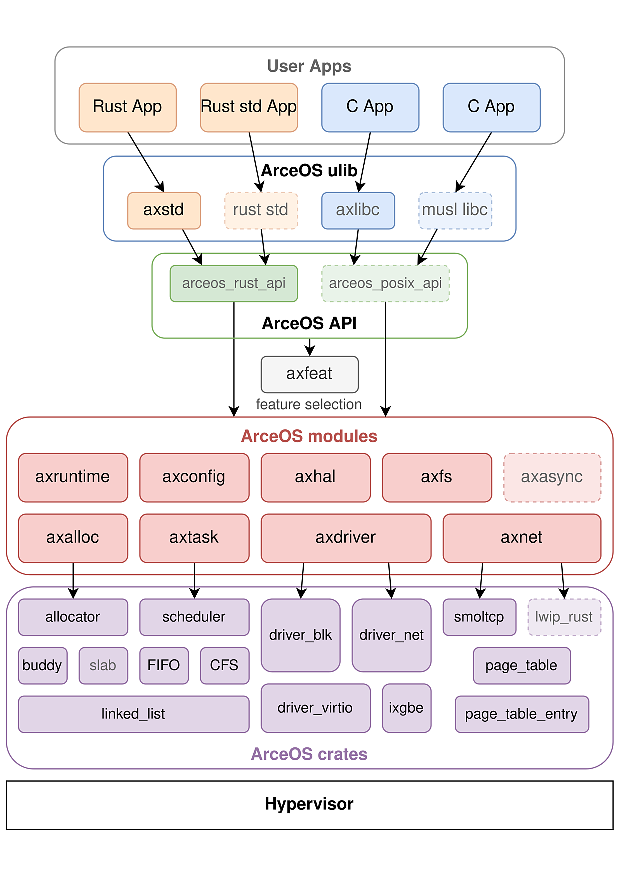
\includegraphics[width=0.5\linewidth]{ArceOS (1).pdf}
  \caption{ArceOS 内核结构图}
  \label{fig:ArceOS}
\end{figure}

每个模块包含多个组件,不同模块组合组合为应用程序提供底层支持。其中应用运行时模块
(axruntime)、硬件抽象层模块(axhal)以及动态内存分配模块(axalloc)是不可缺少的核心组件,
其他模块可以根据具体需求进行选择和使用。

在 ArceOS 的启动过程中,axhal 模块会将对应架构的 \_start 函数链接到 ".text.boot" 段, 作为 ArceOS 运行的第一段代码,完成一些基础的硬件相关初始化操作,例如设置栈指针、初始化页表和 MMU(内存管理单元)等,并跳转到 Rust 主函数 rust\_entry。
rust\_entry 函数位于 axruntime 模块中,它会依据不同的 Cargo 特性进行有针对性的初始化工作,若启用日志功能,会初始化日志系统;启用内存分配特性时,会查找物理内存区域并初始化全局内存分配器;接着会进行平台设备初始化,确保硬件正常工作。对于多任务、文件系统、网络、图形显示、对称多处理以及中断等特性,也会分别完成调度器、设备驱动、从 CPU、中断处理程序等的初始化。最后,它会调用应用的 main 函数,开启应用程序的执行,为操作系统和应用程序的运行构建起完整的基础环境。

当应用程序的 main 函数执行完毕后,若启用了 multitask (多任务)特性,将会调用 axtask::exit(0) 退出函数来退出当前任务;若未启用该特性,则会调用 axhal 模
块下的 misc::terminate 函数来结束整个系统的运行。

\section{ArceOS 内存管理组件及接口}
在 ArceOS 的模块中,axhal、axalloc、axmm 和 axdma 模块是 ArceOS 内存管理的核心模块,它们分别负责对不同硬件平台的硬件封装、物理内存分配、虚拟内存管理和直接内存访问,组成了如图~\ref{fig:ArceOS-mm} 所示的内存管理系统。

\begin{figure}
  \centering
  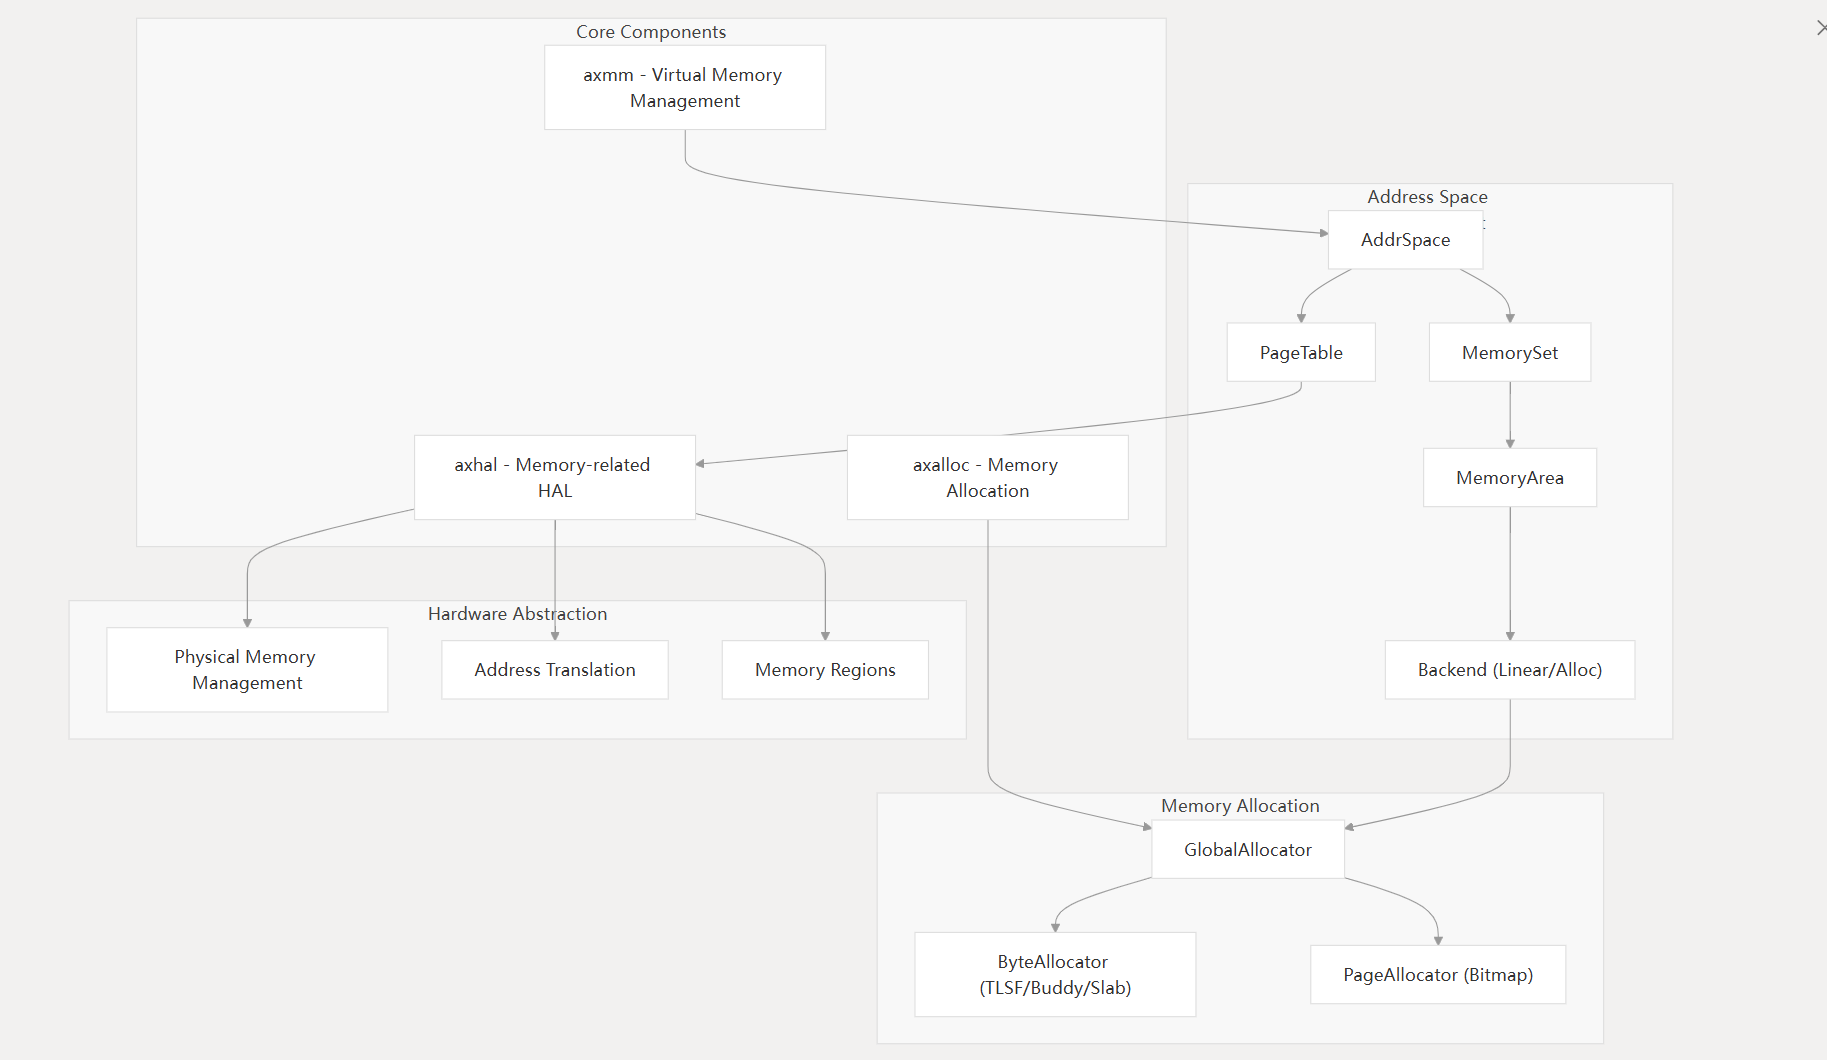
\includegraphics[width=1\linewidth]{arch.png}
  \caption{ArceOS 内存管理系统}
  \label{fig:ArceOS-mm}
\end{figure}

\subsection{axhal}

axhal 组件提供了一层针对不同硬件平台的硬件封装,它为指定的操作平台进行引导和初始化过程,并提供对硬件的操作。在内存方面,axhal 同样进行了一系列的封装操作来支持内存管理。例如:

\begin{itemize}
\item 页表管理封装:axhal 模块将不同架构的页表统一封装为 PageTable 类型,并提供了一致的操作接口,
例如 alloc\_frame(通过页表分配物理页帧)、dealloc\_frame(通过页表释放物理页帧)、phys\_to\_virt(将物理地址转换为虚拟地址)、set\_kernel\_page\_table\_root(设置内核页表根地址)和kernel\_page\_table\_root(获取内核页表根地址)等。
\item 内存区域封装:axhal 模块中定义了 MemRegion 结构体,用于表示和架构无关物理内存区域。MemRegion 结构体包含起始物理地址、区域大小、区域标志和区域名称等属性。通过该结构体,可以方便地管理和操作物理内存区域。
\item 获取内存区域的函数封装:axhal 提供 kernel\_image\_regions、default\_mmio\_regions、default\_free\_regions 接口用于获取内核映像区域、默认 MMIO 区域和默认空闲区域的内存区域列表,并将其封装为 MemRegion 类型。默认的 MMIO 区域和默认空闲区域的位置由 axconfig 模块定义,在不同的硬件平台上可能会有所不同。
\end{itemize}

\begin{figure}
  \centering
  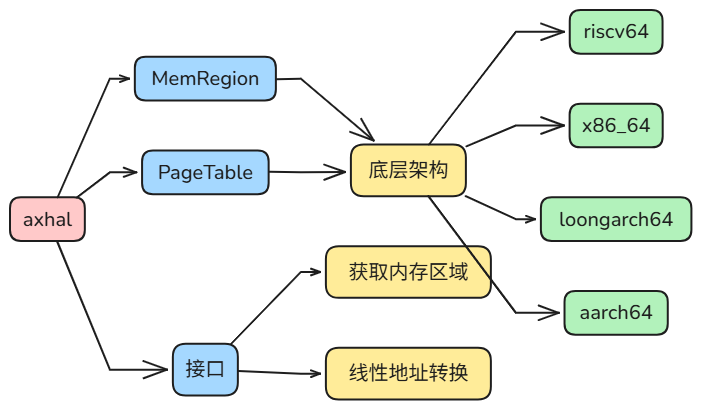
\includegraphics[width=1\linewidth]{axhal-arch.png}
  \caption{axhal 内存管理相关结构图}
  \label{fig:axhal-arch}
\end{figure}



\subsection{axalloc}

\begin{figure}
  \centering
  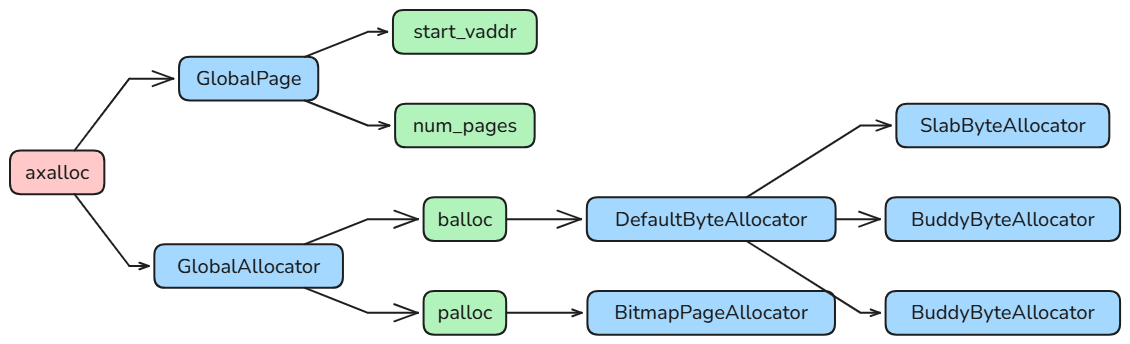
\includegraphics[width=1\linewidth]{axalloc-arch.png}
  \caption{axalloc 结构图}
  \label{fig:axalloc-arch}
\end{figure}

如图\ref{fig:axalloc-arch},axalloc 模块中定义了全局内存分配器 GlobalAllocator,由字节分配器和页面分配器组成。其中,字节分配器用于小内存块的分配和释放,在 ArceOS 中我们提供了三种不同的字节分配器:
\begin{itemize}
\item SlabByteAllocator——基于 slab 分配算法的字节分配器,其核心思想是将内存按照对象的大小进行分类,对于每一类对象,预先分配好一组连续的内存块,这些内存块组成一个 “slab”。每个 slab 包含了多个相同大小的对象槽(Object Slots),当需要分配某个特定大小的对象时,就从对应的 slab 中获取一个空闲的对象槽;当对象释放时,对应的对象槽又可以被重新利用。同时,为了更好地管理这些 slab,会有 slab 缓存(Slab Cache)机制,用于跟踪空闲和已使用的 slab 等状态。
slab 算法对于频繁分配和释放相同类型、相同大小对象的场景表现卓越,同类型对象集中存放使得在数据访问时对 CPU 缓存的利用更为充分,并且可以有效地减少内存碎片。但固定大小的 slab 可能会导致内存浪费和对于多样化、大小不一的内存分配需求适应性较差的问题。
\begin{figure}
  \centering
  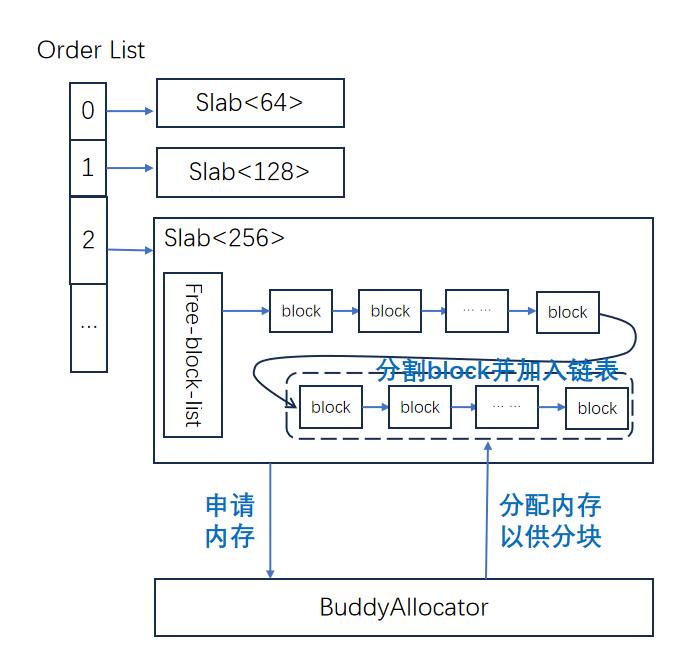
\includegraphics[width=0.7\linewidth]{Slab.png}
  \caption{Slab 算法示意图}
  \label{fig:Slab}
\end{figure}
\item BuddyByteAllocator——基于 Buddy 算法的字节分配器,以一种二叉树的思想来管理内存,它将整个内存空间看作是一个完整的、大小为 2 的幂次方的内存块,当需要分配内存时,如果有符合要求大小(同样是 2 的幂次方)的空闲内存块,就直接分配;若没有,则将更大的空闲内存块不断地二等分(即找到它的 “buddy”,也就是相邻且同样大小的另一半内存块),直到得到合适大小的内存块进行分配。在内存释放时,会检查释放的内存块与其 buddy 是否都空闲,如果是,则将它们合并成一个更大的空闲内存块,如此不断向上合并,直到不能合并为止。
Buddy 算法通过不断地合并空闲的 “伙伴” 内存块,能让内存空间保持相对规整,避免出现大量零散的小空闲块,内存释放时的合并操作判断和执行合并的过程也相对简单高效,但内存分配粒度受限于 2 的幂次方,可能会导致内存浪费和内部碎片问题。
\begin{figure}[H]
  \centering
  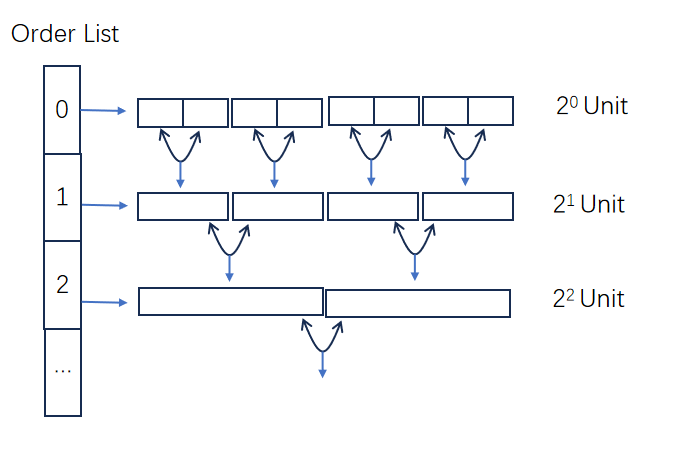
\includegraphics[width=0.7\linewidth,]{Buddy.png}
  \caption{Buddy 算法示意图}
  \label{fig:Buddy}
\end{figure}
\item TlsfByteAllocator——基于 TLSF(Two-Level Segregate Fit)算法的字节分配器,TLSF 采用了两级的分离适配结构。第一级是将整个内存空间按照不同大小范围划分成多个区间,每个区间对应着不同大小的内存块类别,形成一个区间链表。第二级则是针对每个区间,再使用一个位图(Bitmap)和一个空闲块链表来管理该区间内具体的空闲内存块。在进行内存分配时,先根据要分配的内存大小确定所属的区间,然后在位图中查找是否有合适的空闲块,若有则从对应的空闲块链表中取出进行分配;内存释放时,将释放的内存块重新插入到对应的空闲块链表,并相应更新位图信息。
TLSF 算法具有高效的分配速度和高内存利用率,可以灵活应对各种不同大小内存块的分配情况,但是维护两级结构中的各种管理信息使得内存开销相对较大。
\begin{figure}[H]
  \centering
  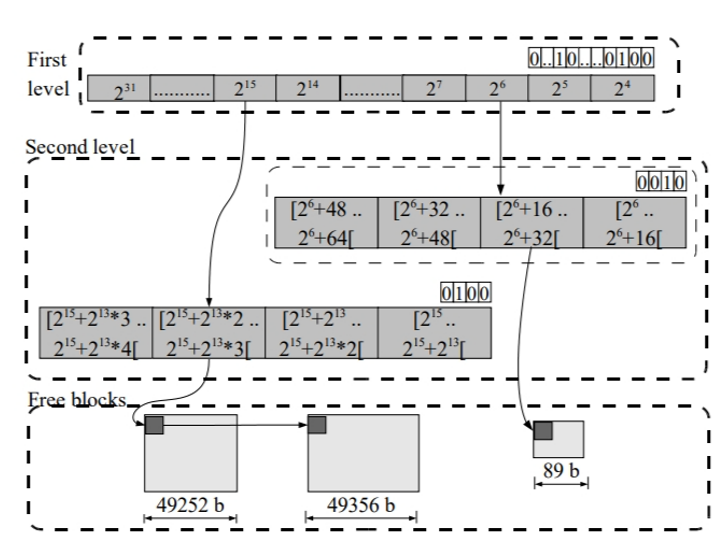
\includegraphics[width=0.7\linewidth]{TLSF.png}
  \caption{TLSF 算法示意图}
  \label{fig:TLSF}
\end{figure}
\end{itemize}

页分配器负责大型分配和扩展字节分配器,使用了标准库中的 BitmapPageAllocator,它是一个基于位图(bitmap)的页粒度内存分配器。它通过使用位图中的每一位来表示一个内存页的分配状态,从而实现高效的内存管理。该分配器支持不同大小的内存分配(从256MB到1TB),并且可以处理不同页大小(PAGE\_SIZE)的情况,要求页大小必须是2的幂次方。它提供了初始化内存区域、分配和释放内存页等基本功能,同时支持对齐分配和指定地址分配等特性。

全局内存分配器通过接口函数提供了对物理内存的操作功能,包括内存的分配、释放、查询等。其主要功能如下:
\begin{itemize}
\item 内存分配器类型选择:通过 Cargo 特性,axalloc 支持用户可以根据需求在 Buddy 分配器、Slab 分配器、TLSF 分配器中选择一种作为全局内存分配器的字节分配器部分。
\item 全局内存分配器初始化:axalloc 定义了一个静态全局变量 GLOBAL\_ALLOCATOR,
并实现了 core::alloc::GlobalAlloc 特性,将其注册为标准库的默认分配器。
在初始化时,需要调用global\_init函数,该函数会初始化页分配器和字节分配器。
\item 内存分配与释放:包括字节分配和释放、页面的分配和释放。
\item 内存状态查询:axalloc 提供了一些函数用于查询内存分配器的状态,如当前内存使用量、空闲内存量等。
\end{itemize}

另外,axalloc 模块提供了用于管理全局内存页面的类型 GlobalPage,其属性包括起始地址和包含的页数。并在全局内存分配器的支持下,提供分配单页和连续页面、填充页面等接口。同时,通过实现 Drop 特性,确保在 GlobalPage 被销毁时,自动释放其占用的内存。这种机制确保了内存资源的高效利用,避免了内存泄漏。

\subsection{axmm}

使用 axalloc 模块提供的内存管理功能,我们已经可以构建起一个简单的内存管理系统,支持内核和应用程序都处于同一地址空间,并且相互可见。
但是,在多任务或多进程的环境下,内核和应用程序之间的内存隔离是非常重要的。为了实现这一点,ArceOS 引入了 axmm 模块来实现虚拟内存管理,其结构如图所示。

\begin{figure}
  \centering
  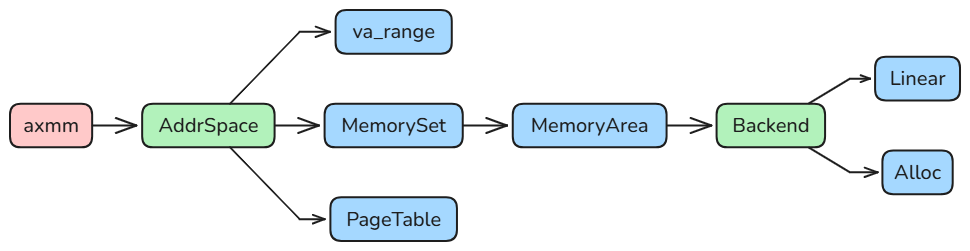
\includegraphics[width=1\linewidth]{axmm-arch.png}
  \caption{axmm 结构图}
  \label{fig:axmm-arch}
\end{figure}


axmm 模块的核心是 AddrSpace 结构体,它表示一个虚拟内存地址空间,包含虚拟地址范围、内存区域集合以及页表。通过该结构体提供的接口,可以对虚拟内存地址空间进行管理,包括创建、映射、解除映射、读写数据等操作。
AddrSpace 的具体接口如图\ref{fig:AddrSpace}所示:
\begin{figure}
    \centering
    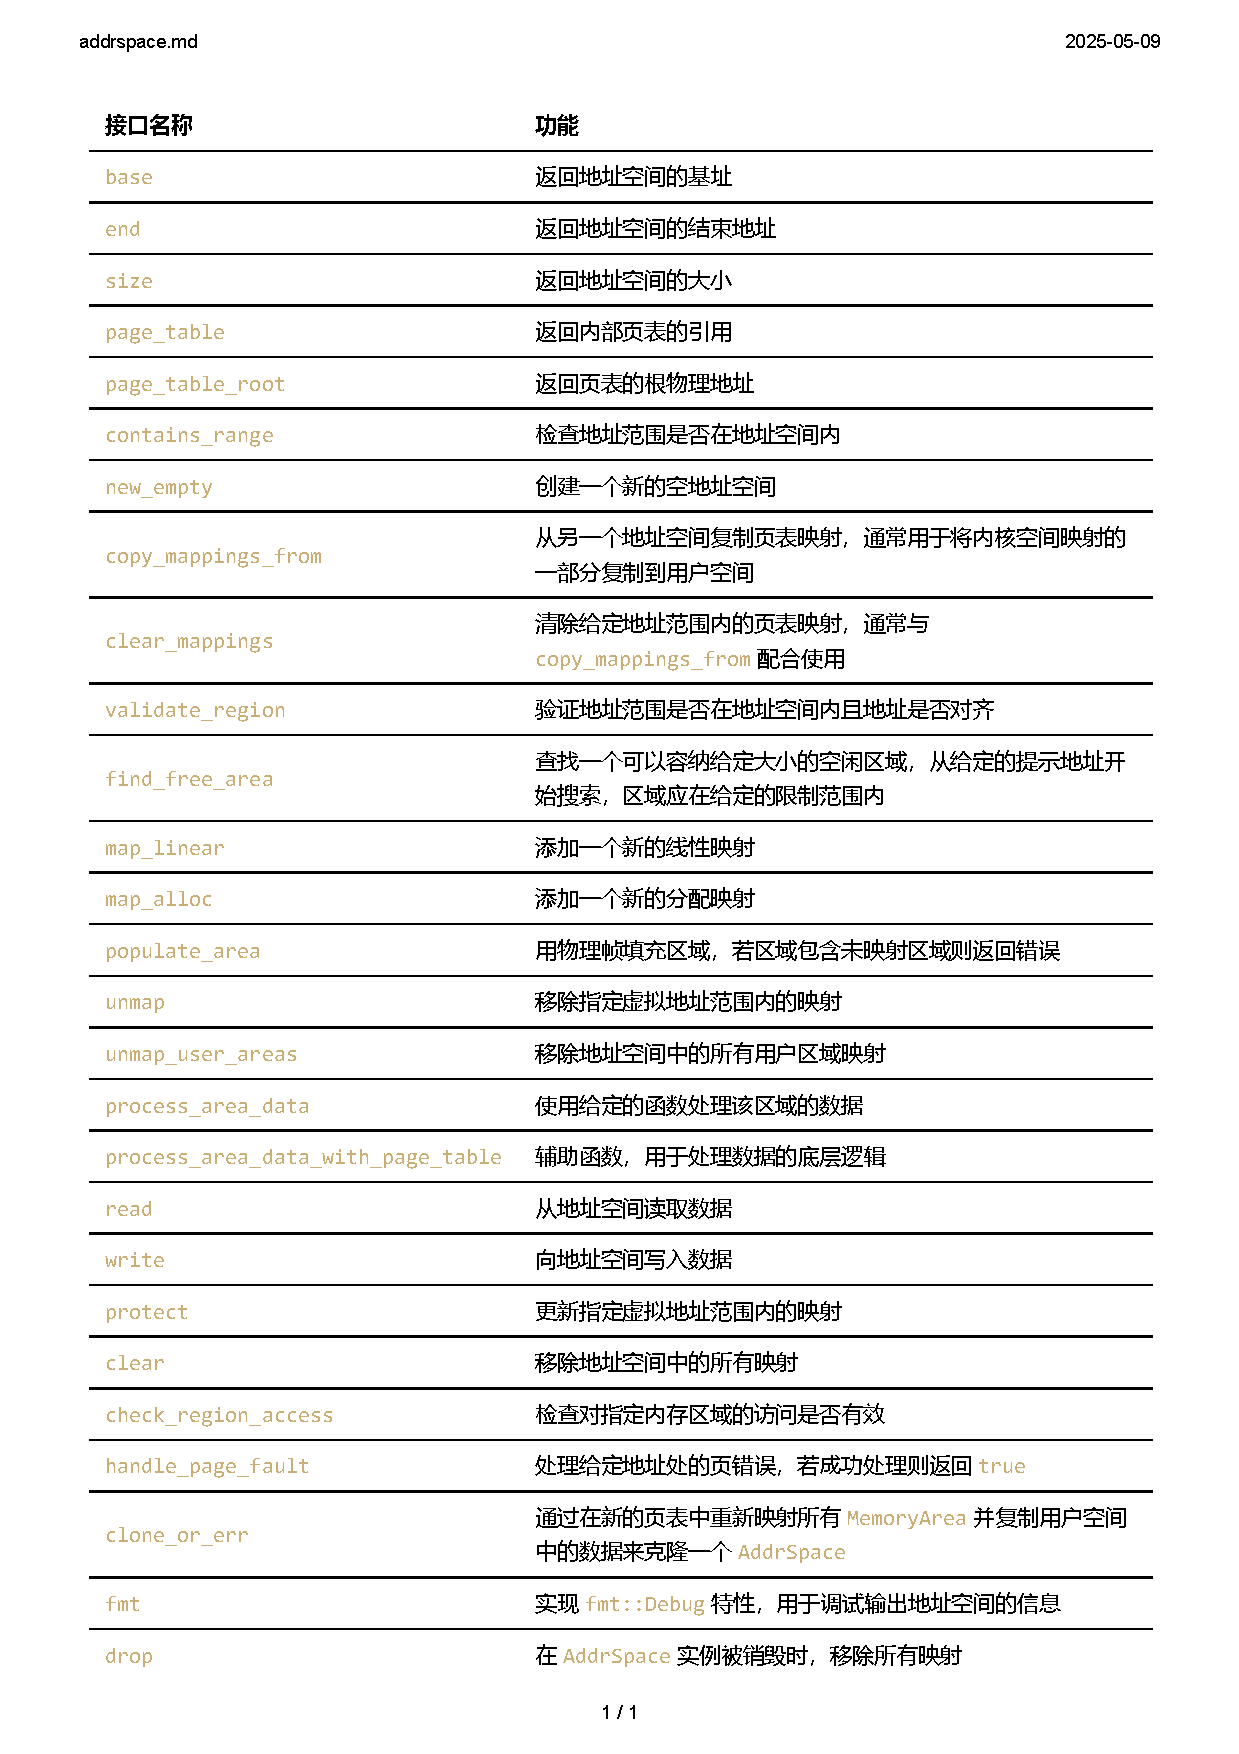
\includegraphics[width=1\linewidth]{addrspace.pdf}
    \caption{AddrSpace 结构体接口}
    \label{fig:AddrSpace}
\end{figure}

实现 AddrSpace 结构体及其接口对于构建一个高效、灵活且安全的虚拟内存管理系统具有极其重要的意义。一方面,通过为每个进程分配独立的虚拟地址空间,AddrSpace 不仅实现了内核与用户空间的隔离,还确保了进程之间的相互独立,从而防止了进程间的非法访问和潜在的破坏行为。

另一方面,AddrSpace 提供的内存保护机制进一步增强了系统的安全性。它通过页表和访问权限控制,确保每个进程只能访问自己被授权的内存区域,同时在检测到非法访问时能够及时触发异常并进行处理,从而避免系统崩溃。这种机制不仅保护了内核的稳定性,还为用户程序提供了可靠的运行环境。

除 AddrSpace 结构体及其接口外,axmm 模块还定义 Backend 核心抽象,用于处理不同类型的内存映射实现细节。它作为 MemoryArea (内存区域)的后端,将虚拟地址与物理存储关联起来,将映射、解除映射、处理页面异常等操作传递到具体的后端实现,进而完成对页表的操作。axmm 模块支持两种类型的内存映射后端:
\begin{itemize}
\item Linear Backend:用于与已知物理地址的直接映射,例如内存映射的 I/O 区域或内核映像部分,虚拟地址和物理地址具有固定的偏移关系;
\item Allocation Backend:按需分配物理页,支持延迟分配,常用于用户空间内存管理。
\end{itemize}

内存区域对应的映射类型在内存区域对象创建时,即调用 AddrSpace 的 map\_linear 或 map\_alloc 方法申请空间并进行映射时指定。

\subsection{axdma}
axdma 模块实现了 DMA 内存管理,提供了直接内存访问的接口。DMA(Direct Memory Access,直接内存访问) 是一种硬件特性,允许某些硬件子系统在不经过 CPU 控制的情况下直接访问系统内存,
DMA 通常用于高速数据传输,例如从硬盘读取数据到内存,或者从内存将数据发送到网络接口。

在传统的数据传输中,CPU 需要逐字节地从外设读取数据,然后将其写入内存,或者从内存读取数据后写入外设。这种操作不仅效率低下,还会占用大量的 CPU 时间。而 DMA 允许外设直接访问内存,
无需 CPU 参与,从而提高了数据传输的速度和效率,并释放了 CPU 的计算资源,使其可以处理其他任务。

\begin{figure}[H]
    \centering
    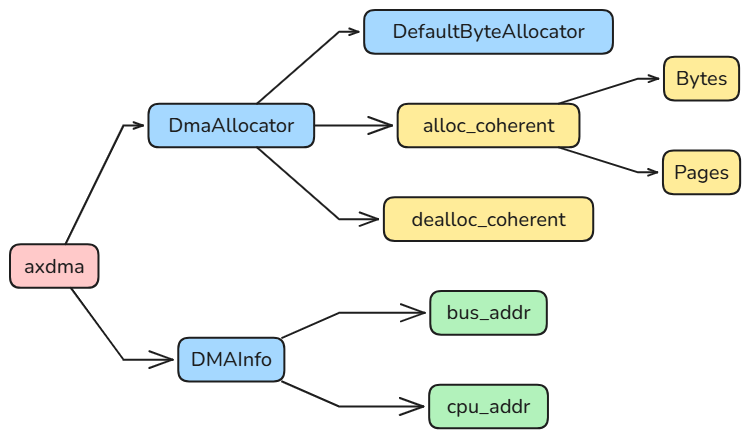
\includegraphics[width=1\linewidth]{axdma-arch.png}
    \caption{axdma 结构图}
    \label{fig:axdma-arch}
\end{figure}

如图\ref{fig:axdma-arch},ArceOS 的 DMA 模块通过实现 DMA 分配器(DmaAllocator),向设备驱动模块(axdriver)提供了 DMA 内存分配和释放的接口。
它会根据设备的需求,分配合适大小的内存块,并在 DMA 操作完成后释放这些内存块。
DMA 分配器还会处理 DMA 操作中的地址转换问题,将虚拟地址转换为总线地址,以便于 CPU 访问。
DMAInfo 结构体则记录了用于 DMA 操作的内存区域相关的信息,包括 CPU 访问该区域的虚拟地址和该区域在总线上的物理地址。
同时,DMA 分配器分配的内存需要标记为 UNCACHED,以避免缓存一致性问题,这需要虚拟内存管理模块(axmm)提供的接口来完成。

DMA 模块的具体接口如图\ref{fig:DmaAllocator}所示:
\begin{figure}[H]
    \centering
    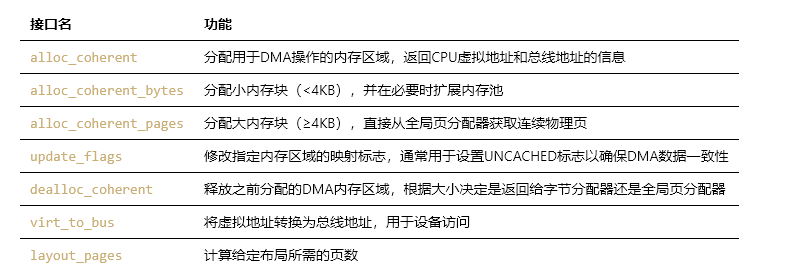
\includegraphics[width=0.7\linewidth]{axdma.png}
    \caption{DmaAllocator 结构体接口}
    \label{fig:DmaAllocator}
\end{figure}

\section{ArceOS 内存管理机制}

% ArceOS 中与内存管理相关的结构主要有:

% \begin{itemize}
% \item MemRegion:表示一个物理内存区域,包含起始物理地址、区域大小、区域标志和区域名称。
% \item GlobalAllocator:全局内存分配器,用于管理物理内存区域,包含用于小分配的字节分配器和用于大型分配和扩展字节分配器的页分配器,提供了内存和页面的分配和释放接口。
% \item AddrSpace:表示虚拟内存地址空间,包含虚拟地址范围、内存区域集合以及页表。通过该结构体提供的接口,可以对虚拟内存地址空间进行管理,包括创建、映射、解除映射、读写数据等操作。
% \item MemoryArea:表示一块虚拟内存区域,包含起始地址、结束地址、访问权限和映射关系等信息。
% \item MemorySet:表示虚拟内存区域的集合构成的 Btree 结构,提供管理虚拟内存区域的具体方法。
% \item Backend:内存映射后端,包括 Linear Backend 和 Allocation Backend。
% \end{itemize}

在本章第一节中我们提到了 ArceOS 的启动和初始化过程,而在这里我们将对其中与内存分页相关的部分进行详细分析:
架构的初始化函数 \_start 中进行了启动页表和内存管理单元的初始化,为 QEMU 虚拟机的物理内存等关键区域构建映射,设置根页表地址并刷新 TLB,完成分页的早期启动阶段。
这一阶段是 ArceOS 默认开启的,构建的映射为恒等映射,虚拟地址和物理地址相同,主要用于内核的启动和初始化。
\begin{lstlisting}[language=c, caption=\_start]
phys_virt_offset = const PHYS_VIRT_OFFSET,
boot_stack_size = const TASK_STACK_SIZE,
boot_stack = sym BOOT_STACK,
init_boot_page_table = sym init_boot_page_table,
init_mmu = sym init_mmu,
\end{lstlisting}

如图~\ref{fig:init}所示,分页的早期启动阶段完成后,如果开启了 paging 特性,在 rust\_main 函数中会调用 axmm 模块的 init\_memory\_management 函数初始化内存管理,
即创建内核的虚拟地址空间,为内核的虚拟地址空间构建线性映射,调用 axhal 的接口设置内核的虚拟地址空间的页表,并将其设置为当前的页表根,完成分页的重建映射阶段。
该阶段将内核和用户空间的虚拟地址空间隔离开来,让内存管理模块能够管理更大的地址空间,为 DMA 和多任务等功能提供支持。

\begin{figure}[H]
    \centering
    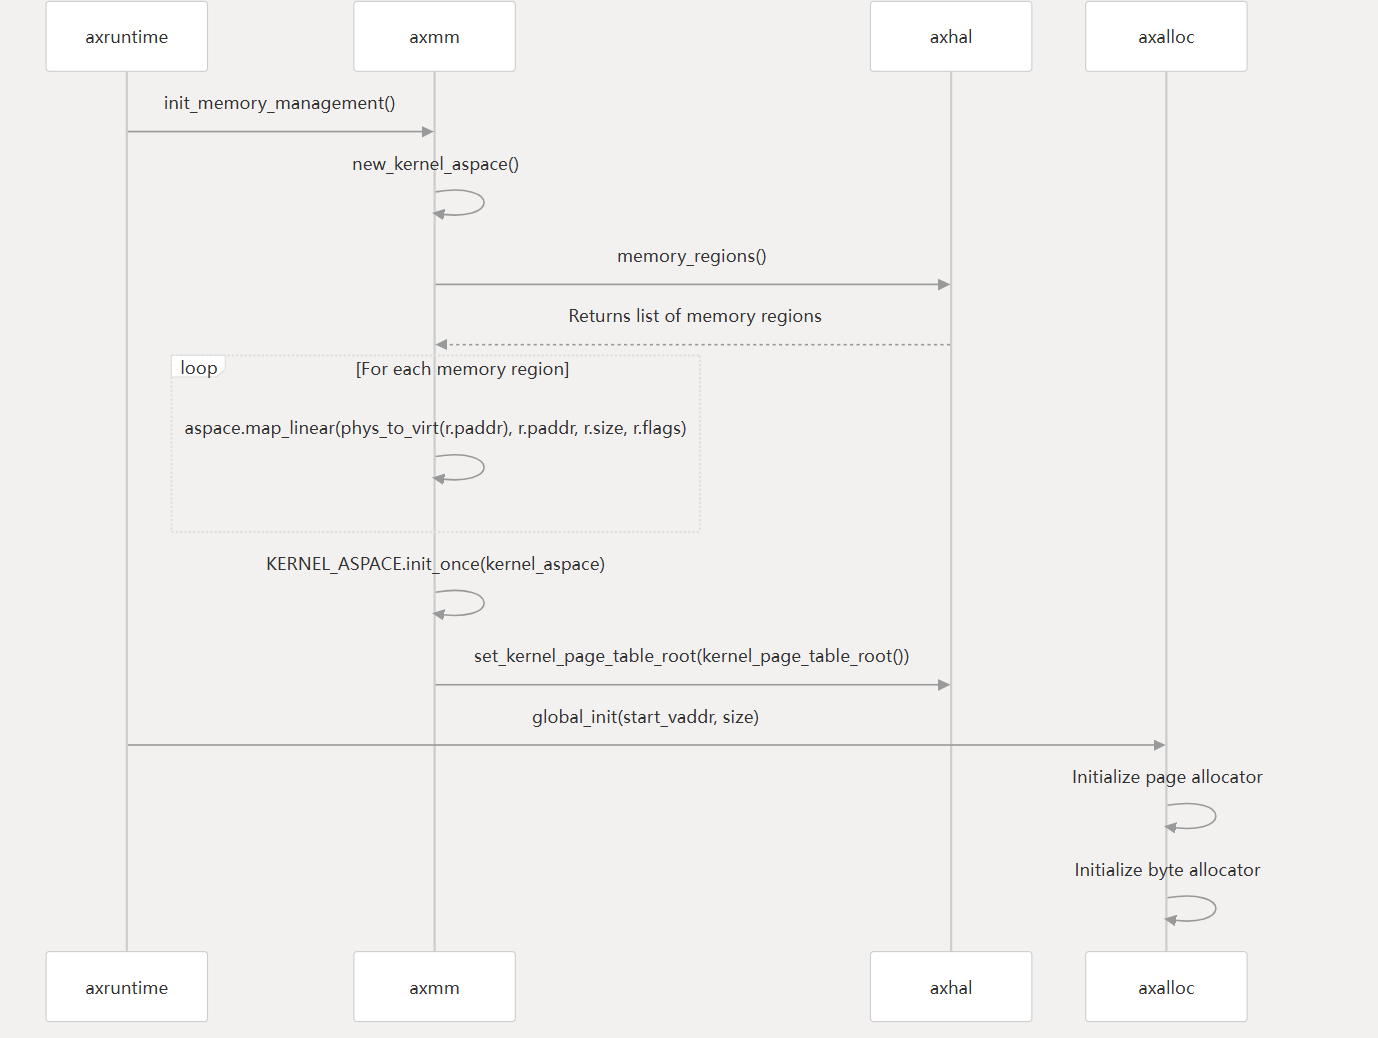
\includegraphics[width=1\linewidth]{init.png}
    \caption{分页的重建映射阶段}
    \label{fig:init}
\end{figure}

开启 paging 特性且上层架构或者应用需要对内存空间进行操作时,会调用 AddrSpace 的相应接口,如 find\_free\_area(寻找空闲内存区域)、map\_linear(建立线性映射)、map\_page(建立分配映射)等方法,这些方法会根据具体的内存操作需求,对页表和虚拟地址空间进行操作,并调用全局内存分配器进行物理内存的分配和释放。全局分配器在分配时会先尝试从字节分配器分配,如果字节分配器内存不足,则计算需要多少内存,从页面分配器分配页面后将页面添加到字节分配器重新进行分配,此方法允许高效处理小型和大型分配,同时保持合理的内存使用率。

同时,ArceOS 还在 AddrSpace 结构体中提供了页面异常的处理接口,例如当访问的虚拟地址对应的物理页不存在时,会触发缺页异常,此时会调用 AddrSpace 的 handle\_page\_fault 函数处理缺页异常,
该函数会对后端为 Alloc 类型的地址,调用 axalloc 中的全局内存分配器进行物理页的分配,并通知 axhal 中的页表更新映射关系。对于后端为 Linear 类型或者需要填充的地址,则会处理失败,返回 false,
因为这两类的地址在创建时就应完成物理页的分配和映射,缺页异常的处理不适用。AddrSpace 的 handle\_page\_fault 函数的流程图如图~\ref{fig:handle-page-fault-arceos}所示:

\begin{figure}[H]
    \centering
    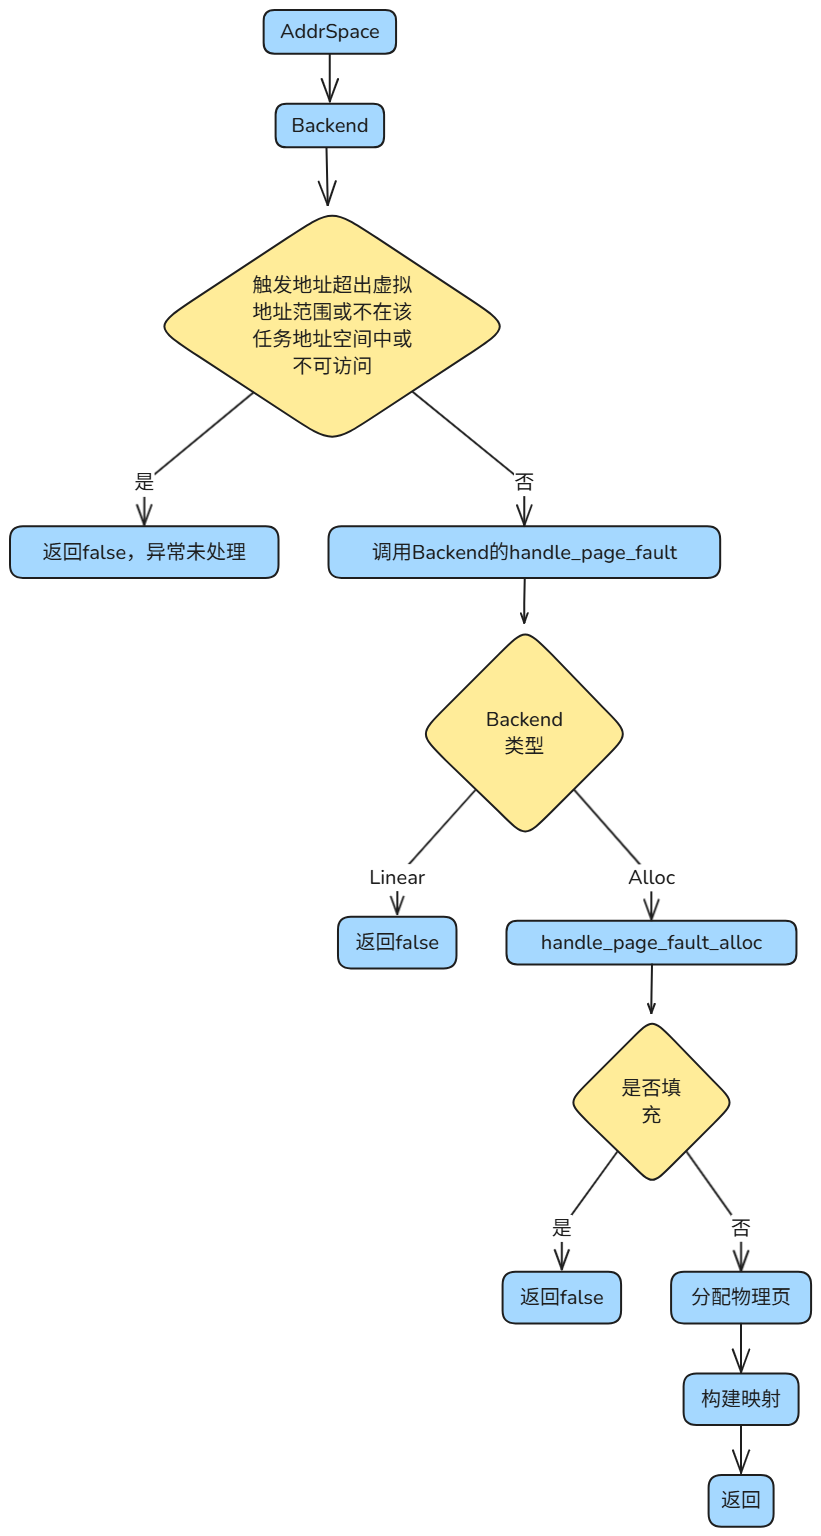
\includegraphics[width=0.7\linewidth]{pagefault-arceos.png}
    \caption{handle\_page\_fault 函数流程图}
    \label{fig:handle-page-fault-arceos}
\end{figure}


借助缺页异常的处理,ArceOS 还实现了 Lazy Map 机制,即当访问的虚拟地址对应的物理页不存在时,不会立即分配物理页,而是在第一次访问该虚拟地址时才触发缺页异常,进行分配和映射。
% !TeX root = ../cyh.tex

\chapter{starry-next 宏内核}

\section{starry-next 宏内核整体架构}

Starry-next (StarryOS) 是构建在 ArceOS 基础之上的操作系统内核。它实现了一个兼容 Linux 的系统调用接口,同时支持多种硬件架构,包括 x86\_64、riscv64、aarch64 和 loongarch64。

代码结构上,Starry-next 主要由以下模块组成:

\begin{itemize}
\item core:基于 ArceOS 的底层支持实现 StarryOS 的核心内核功能,包括内存管理(mm)、任务管理(task)和时间管理(time)等。其中内存管理模块负责分配、释放和映射,如 copy\_from\_kernel 函数用于将内核空间的映射复制到用户地址空间,load\_user\_app 函数用于加载用户应用程序到内存中。任务管理模块处理任务和线程的创建、调度和管理,例如 new\_user\_task 函数用于创建新的用户任务。时间管理模块管理系统时间和定时器。
\item api: 现面向用户的 API 和系统调用接口,涵盖文件系统操作、进程管理、线程管理、内存管理等多个方面。
\item src:主要负责启动主函数、加载应用程序并对系统调用的分发进行处理。
\item 其他:包括用于适配不同架构的配置文件和工具链,以及用于构建和运行 StarryOS 的构建工具和脚本。
\end{itemize}

功能上,Starry-next 也可以划分为较为独立的模块:

\begin{itemize}
\item 内存管理模块:负责管理物理内存和虚拟内存,包括内存分配、映射和释放等操作。
\item 进程管理模块:负责管理进程和线程,包括进程创建、调度和管理等操作。
\item 文件系统模块:负责管理文件系统,包括文件的创建、读取、写入和删除等操作。
\item 网络模块:负责管理网络操作,包括网络协议栈、网络设备驱动等操作。
\item 系统信息模块:负责提供系统信息和状态,包括 CPU、内存、网络等信息。
\item 信号模块:负责处理信号和中断,包括信号的发送、接收和处理等操作。
\end{itemize}

每个功能模块都需要向应用程序提供相应的系统调用接口,为应用程序提供内核服务。同时,功能模块还需要尽可能复用 ArceOS 的底层组件和接口,以减少代码的重复和维护成本。
功能模块之间通过明确定义的接口进行通信,确保系统的稳定性和可拓展性。

通过结构和功能上的划分与解耦,Starry-next 宏内核的每个模块都可以独立开发、测试和维护,增强了系统的可拓展性和稳定性,也使得本课题大方向上的多名开发者可以在同一代码库上进行协作开发。

\begin{figure}[H]
    \centering
    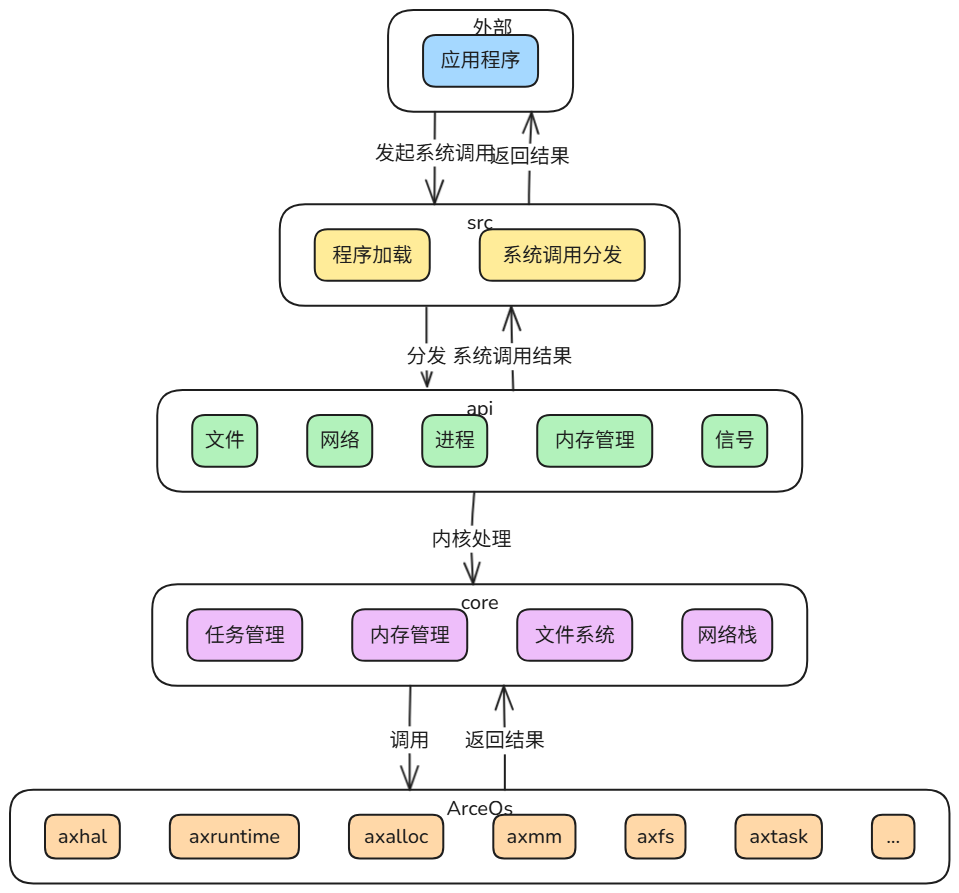
\includegraphics[width=0.7\linewidth, keepaspectratio]{starry-arch.png}
    \caption{starry-next 宏内核架构}
    \label{fig:starry-next}
\end{figure}

\section{starry-next 初始化和运行过程}

% Starry-next 以 main 函数作为系统的入口点,创建初始化进程,为环境变量指定的测试用例创建用户应用程序,并依次运行这些应用程序。在运行过程中,Starry-next 会根据系统资源的需求,动态地分配和管理内存,同时处理各种系统调用,如 fork、exec、wait、mmap、munmap 等。

starry-next 的初始化从 Bootloader 将控制权交给内核入口点开始,之后 ArceOS 的 axhal 模块和 axruntime 模块会完成硬件的初始化,并根据选择的特性进行内存管理器、任务管理器、文件系统、网络等模块的初始化。接着,axruntime 模块以 src 中 main 函数创建一个初始化进程,进而为环境变量指定的测试用例创建用户应用程序,并将用户程序加载到内存中。

% 在运行过程中,starry-next 会根据系统资源的需求,动态地分配和管理内存,同时处理各种系统调用,如 fork、exec、wait、mmap、munmap 等。这些系统调用会使操作系统内核进入内核态,执行 core 中相应的处理程序,并调用底层的 ArceOS 提供的接口进行处理。
% 最后的处理结果将返回系统调用层,进而返回给用户空间的应用程序。

在运行过程中,starry-next 会逐个运行应用程序,并根据系统资源的需求,动态地分配和管理内存。
当应用程序发起系统调用时,先由 src 层将参数根据系系统调用号分发到 api 层的相应处理函数,
api 层的函数会检查参数的类型、取值范围等是否符合系统调用的规范。验证参数无误后,api 层函数会根据系统调用的具体功能,调用 core 层的相关功能模块及其底层的 ArceOS 组件来完成实际的操作。
当 core 层完成操作并返回结果后,api 层会对返回结果进行处理。如果操作成功,api 层会将结果按照系统调用的约定进行封装,以便返回给应用程序。如果操作失败,api 层会根据错误类型设置合适的错误码。
最后,api 层的函数会将处理结果返回给 src 层,src 层会将结果返回给应用程序。

\begin{figure}[H]
    \centering
    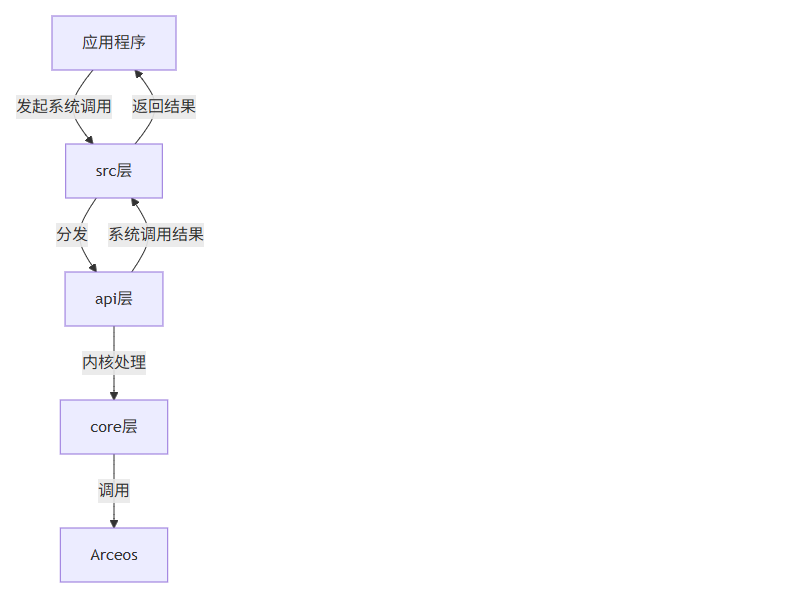
\includegraphics[width=1\linewidth, keepaspectratio]{syscall.png}
    \caption{系统调用流程}
    \label{fig:syscall}
\end{figure}


\section{starry-next 内存管理模块}

\subsection{模块结构}

\begin{figure}[H]
    \centering
    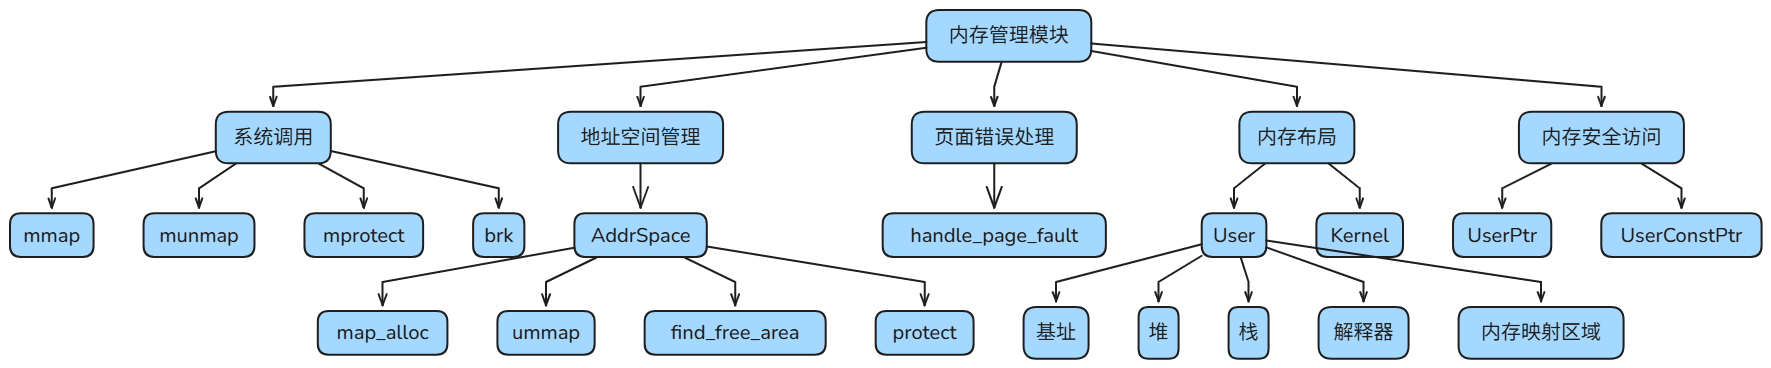
\includegraphics[width=1\linewidth, keepaspectratio]{mm-arch2.png}
    \caption{starry-next 内存管理模块结构}
    \label{fig:mm-arch}
\end{figure}

starry-next 的内存管理模块主要由以下部分组成:

\begin{itemize}
    \item 系统调用:提供了一系列系统调用接口,用于管理内存,如 mmap、munmap、mprotect、brk 等。
    \item 地址空间管理:使用 AddrSpace 结构体及其接口管理用户程序的地址空间,包括内存映射、权限控制等。
    \item 页面异常处理:当用户程序访问内存空间时触发的缺页异常会调用相应的处理函数。
    \item 内存布局:定义了内存布局,包括内核空间和用户空间的划分。
    \item 安全内存访问:通过指针封装提供对用户空间内存的安全访问。
\end{itemize}

\subsection{内存管理机制}

starry-next 的内存管理基本上复用了 ArceOS 的内存管理机制:使用 ArceOS 提供的 AddrSpace 结构体管理用户程序的内存空间,当用户程序需要对内存进行操作时,会调用相应的系统调用,如 mmap、munmap、mprotect、mremap 等,这些系统调用会调用 AddrSpace 结构体的接口在用户地址空间中创建和管理内存映射,同时也会调用全局内存分配器进行物理页的分配和映射。

但作为宏内核,starry-next 需要区分内核态和用户态,因此还对内存管理进行了进一步的优化和扩展,例如为用户态和内核态分别设置了不同的地址空间,并且用户态进程不能直接访问内核态内存空间,
而是需要发出系统调用,通过 trap 机制进入内核态,再进行对应处理,通过这种方式来实现用户态和内核态的隔离;在一些架构中将内核部分的映射复制到用户地址空间,使用户态进程可以直接访问内核的某些数据结构或代码片段,
可以减少内核态和用户态之间的切换开销,提高系统的性能。

\subsection{页面异常处理}
页面异常的处理方面,starry-next 在 ArceOS 的基础上增加了判断:如果是用户态程序访问内存空间或者是内核态程序访问用户内存空间时触发的缺页异常,才会调用用户程序的 handle\_page\_fault 函数,
也就是 ArceOS 的 AddrSpace 结构体提供的页面错误处理函数处理缺页异常,该函数会根据虚拟地址的映射关系,调用全局内存分配器进行物理页的分配和映射。
如果 AddrSpace 结构体不能成功处理该异常,则会打印错误信息并终止当前任务,并发送 SIGSEGV 信号。

\begin{figure}[H]
    \centering
    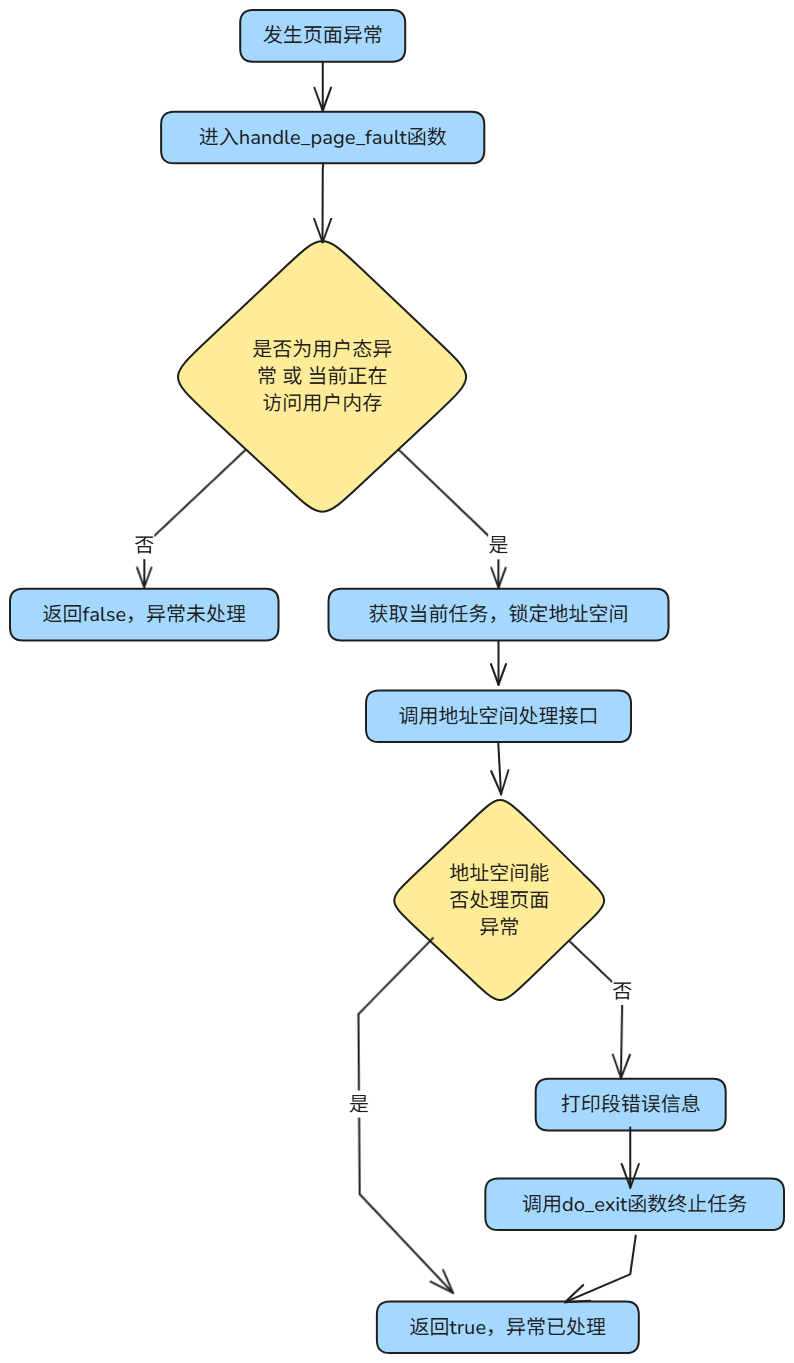
\includegraphics[width=0.7\linewidth, height=14cm,keepaspectratio]{pagefault-starry.png}
    \caption{starry-next 页异常处理}
    \label{fig:pagefault-starry}
\end{figure}

\subsection{内存布局}

不启动 ArceOs 的 paging 特性时,应用和内核在同一空间中运行,系统直接使用物理地址。物理空间的结构如图\ref{fig:phy-layout2}所示。
在 Cargo 项目启动时,axhal 组件的 build.rs 构建文件会根据根据 linker.lds.S 文件中的链接脚本,将物理空间划分为多个部分——内核部分从指定的基地址开始,首先放置可执行代码段(.text),然后是只读数据段(.rodata)和初始化函数数组(.init\_array)。接着是可读写数据段(.data),线程局部存储相关段(.tdata 和 .tbss),以及每个CPU核心的私有数据段(.percpu)。最后是未初始化数据段(.bss),其中包含了启动栈空间,设备内存则位于 0 地址和内核空间之间。整个布局严格遵循4K对齐,并在最后定义了一些与中断处理、系统调用等相关的自定义段。

\begin{figure}[H]
\centering %图片全局居中
%并排几个图,就要写几个minipage
\begin{minipage}[b]{0.45\textwidth} %所有minipage宽度之和要小于1,否则会自动变成竖排
\centering %图片局部居中
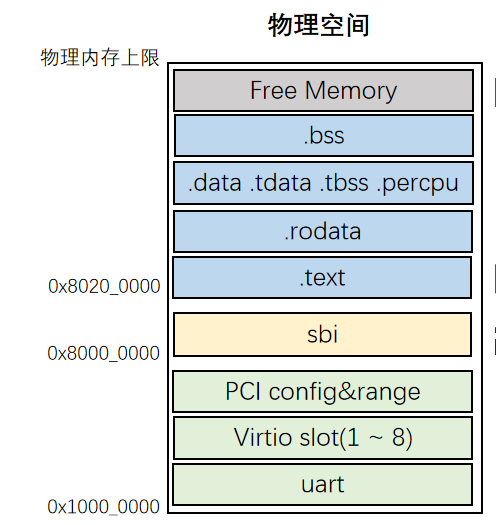
\includegraphics[width=0.8\textwidth]{phy-layout.png} %此时的图片宽度比例是相对于这个minipage的,不是全局
\caption{物理内存布局}
\label{fig:phy-layout2}
\end{minipage}
\begin{minipage}[b]{0.45\textwidth} %所有minipage宽度之和要小于1,否则会自动变成竖排
\centering %图片局部居中
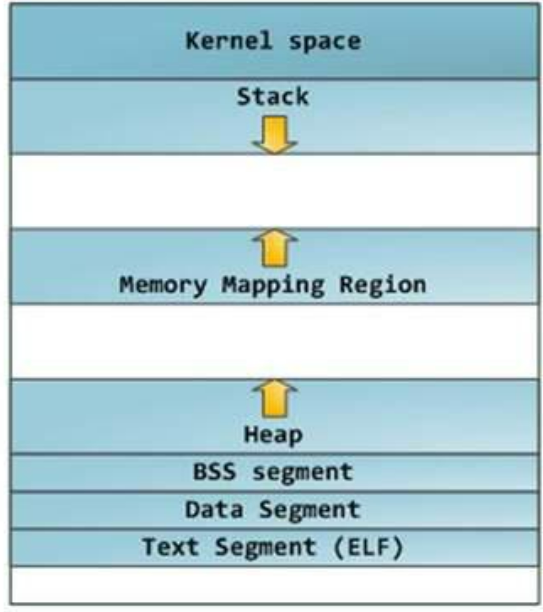
\includegraphics[width=0.8\textwidth]{virt-layout.png}%此时的图片宽度比例是相对于这个minipage的,不是全局
\caption{进程虚拟空间布局}
\label{fig:virt-layout2}
\end{minipage}
\end{figure}


% \begin{figure}[H]
%     \centering
%     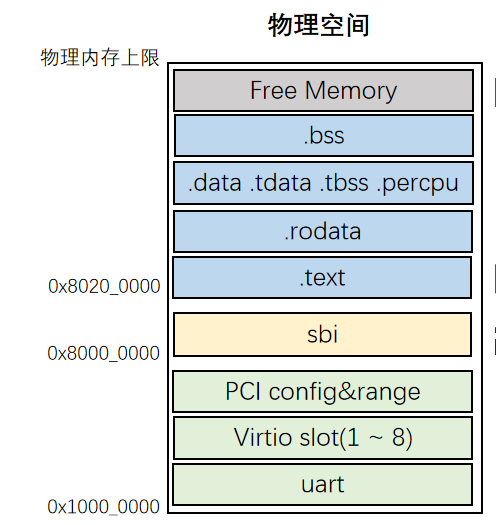
\includegraphics[width=0.5\linewidth, keepaspectratio]{phy-layout.png}
%     \caption{物理内存布局}
%     \label{fig:phy-layout}
% \end{figure}

starry-next 启动了 paging 特性,为每个应用程序分配一个独立的的虚拟地址空间,即 AddrSpace 结构体,用于管理用户程序的内存空间。如图\ref{fig:virt-layout2}所示,进程地址空间分为用户空间和内核空间两部分,用户空间位于低地址,包括了代码段、数据段、堆、栈、内存映射区域。
其中,代码段和数据段是用户程序的只读和读写数据,堆是用户程序的动态内存分配区域,栈是用户程序的函数调用和局部变量存储区域。
内核空间位于高地址,包括了内核代码段、内核数据段、内核堆、内核栈、页表。不同架构下各部分的具体起始地址和大小会有所不同,具体设置可参照表\ref{tab:virt-layout-config}。
% \begin{figure}[H]
%     \centering
%     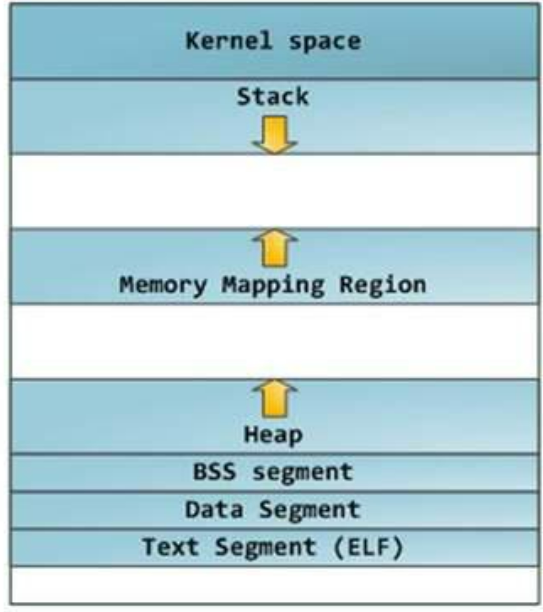
\includegraphics[width=0.5\linewidth, keepaspectratio]{virt-layout.png}
%     \caption{进程虚拟空间布局}
%     \label{fig:virt-layout}
% \end{figure}

\begin{table}[!ht]
    \centering
    \begin{tabular}{lllll}
    \hline
        ~ & x86\_64 & RISC-V 64 & AArch64 & LoongArch64  \\ \hline
        User space base & 0x1000 & 0x1000 & 0x1000 & 0x1000  \\ \hline
        User space size & 128 TB & 4 GB & 128 TB & 4 GB  \\ \hline
        User interpreter base & 64 MB & 64 MB & 64 MB & 64 MB  \\ \hline
        User heap base & 1 GB & 1 GB & 1 GB & 1 GB  \\ \hline
        User heap initial size & 64 KB & 64 KB & 64 KB & 64 KB  \\ \hline
        User stack top & 0x7fff\_0000\_0000 & 0x4\_0000\_0000 & 0x7fff\_0000\_0000 & 0x4\_0000\_0000  \\ \hline
        User stack size & 64 KB & 64 KB & 64 KB & 64 KB  \\ \hline
        Kernel stack size & 256 KB & 256 KB & 256 KB & 256 KB \\ \hline
    \end{tabular}
    \caption{各架构虚拟空间设置}
    \label{tab:virt-layout-config}
\end{table}

\subsection{安全内存访问}

为了保证系统的安全性和稳定性,starry-next 对用户空间内存的访问进行了严格的控制和保护,通过指针封装提供对用户空间内存的安全访问。
具体来说,starry-next 定义了 UserPtr 和 UserConstPtr 两个安全指针类型,分别表示指向用户空间内存的可变和不可变指针。
在访问用户空间内存时,要检查地址是否对齐、当前任务是否有权限访问该地址、地址是否在用户空间范围内并于已经分配映射。
如果这些条件都满足,则可以安全地访问用户空间内存,否则会抛出异常并终止当前任务。

UserPtr 和 UserConstPtr 提供了一系列接口,用于对用户空间内存进行访问和修改。例如:
负责基本信息的查询的 address(获取指针所指向的虚拟地址)和 is\_null(判断指针是否为空)和
获取切片和引用的 get\_as\_mut 和 get\_as\_mut\_slice 等。

\begin{figure}[H]
    \centering
    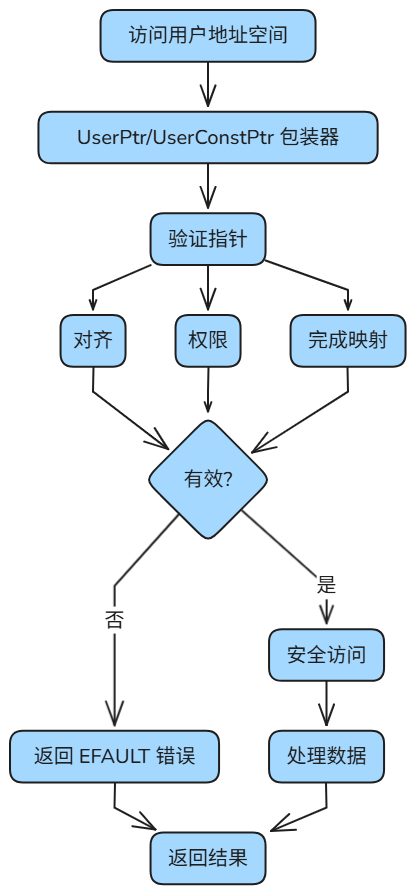
\includegraphics[width=0.5\linewidth]{ptr.png}
    \caption{安全内存访问流程}
    \label{fig:ptr}
\end{figure}
% !TeX root = ../cyh.tex


\chapter{内存管理子系统接口的设计与实现}

\section{内存管理子系统概述}

前两章中我们分别介绍了 ArceOS 基座中的内存管理组件和 starry-next 的内存管理模块,
而本小节则将二者串联起来,从 crate (即 Rust 模块,本节简称为模块)层面介绍内存管理子系统的结构。

\begin{figure}[H]
    \centering
    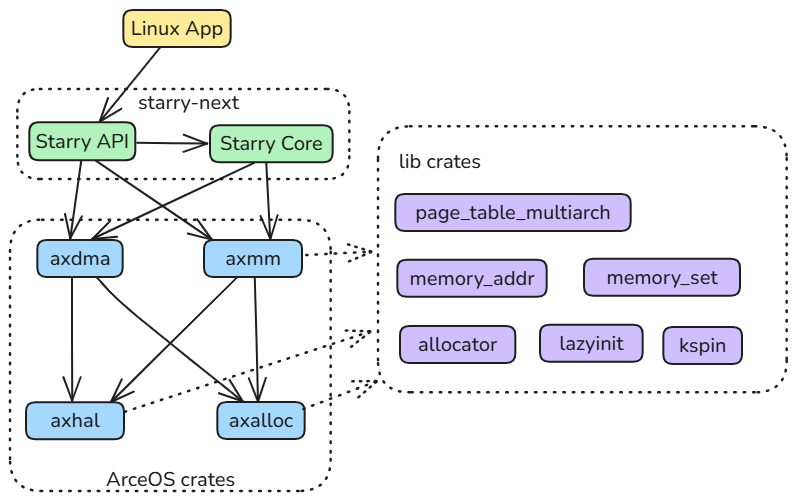
\includegraphics[width=0.7\linewidth, keepaspectratio]{subsystem2.png}
    \caption{内存管理子系统结构图}
    \label{fig:subsystem}
\end{figure}

如图\ref{fig:subsystem}所示,starry-next 中的 API 模块为应该提供系统调用支持,
并根据需要调用 Core 模块中的方法。而在这两个模块的功能又依赖于 ArceOS 中的模块,
例如 axmm 模块提供了内存管理的基本功能,axdma 模块提供了 DMA 相关的功能。
ArceOS 中的模块间也存在相互依赖关系,例如 axmm 和 axdma 依赖 axalloc 提供的全局内存分配器,
并且需要 axhal 提供不同架构的页表抽象相关功能和 axconfig 提供相关配置信息。
在 ArceOS 的下层,是 Rust 和第三方库的支持,例如 page\_table\_multiarch 提供了页表抽象的支持,
memory\_addr 和 memory\_set 提供内存地址和内存集合的抽象,lazyinit 和 kspin 提供了懒初始化和自旋锁的支持等。

内核启动后,先通过 axhal 和 axruntime 进行初始化,包括页表初始化、全局内存分配器的初始化和分配内核空间等。
然后启动 starry-next 的 main 函数,加载用户程序、分配用户空间和通过任务管理子系统进行任务调度。
在用户程序运行过程中,如果需要进行内存分配或释放等操作,则通过 mmap、munmap 等系统调用进入 starry-next 的 API 模块,
进而进入 ArceOS 的 axmm 等模块进行内存管理操作。
任务结束后,任务管理子系统会调用 axmm 等模块进行内存等资源的释放和回收。


\section{内存管理子系统直接相关的系统调用}

\subsection{mmap 系统调用}
mmap 用于将文件或设备内存映射到进程的地址空间。它在 Linux 和类 Unix 系统中广泛使用,主要用于高效地读写文件、实现内存共享以及分配匿名内存等。

mmap 系统调用的原型如下:


\begin{lstlisting}[language=C, caption=mmap 系统调用函数原型]
void *mmap(void addr[.length], size_t length, int prot, int flags, int fd, off_t offset);
\end{lstlisting}



可以看到,mmap 系统调用共有 6 个参数,其中 addr 和 length 用于指定内存映射的起始地址和长度,prot 用于指定内存映射的保护属性,flags 用于指定内存映射的标志,fd 用于指定要映射的文件描述符,offset 用于指定文件偏移量。当 addr 为 NULL 时,表示由内核自动选择内存映射的起始地址。在 Linux 中,内核会选择一个附近的页面边界,并尝试创建映射。如果该地址已经存在另一个映射,内核会选择一个新的地址。flags 参数决定了对映射区域的更新是否对映射同一区域的其他进程可见,以及更新是否会被写入底层文件,例如,MAP\_SHARED 标志表示对映射区域的更新对所有共享该映射的进程可见,而 MAP\_PRIVATE 标志则表示对映射区域的更新对其他进程不可见。

mmap 系统调用的返回值是一个指向内存映射区域的指针,该指针指向映射区域的起始地址。如果调用失败,返回值为 MAP\_FAILED(通常为 -1)。

内存映射主要分为两种类型:匿名映射是指不与任何文件关联的内存映射,通常用于分配动态内存,类似于 malloc,但提供了更多的灵活性和控制能力,例如多个进程可以共享同一个内存映射区域;文件映射是指将文件的内容映射到内存中,这样就可以像访问内存一样访问文件的内容,通常用于实现文件的高效读写。

如图\ref{fig:mmap}所示,在 starry-next 中,mmap 系统调用的实现主要包括以下几个步骤:首先解析参数并检查其有效性;然后进行地址对齐处理,根据是否指定映射起始地址选择将映射长度向上对齐到 4KB (页面大小)或将映射的起始和结束地址分别对齐到页面边界;接着确定映射的真正地址:如果 flag 中设置了 MAP\_FIXED 标志,则使用对齐后的 addr 地址作为映射的起始地址,并且如果 addr 和 length 指定的内存区域与任何现有的映射重叠,那么现有映射的重叠部分将被丢弃,否则,内核会在指定地址附近或者整个用户地址空间中寻找符合条件的空闲地址,并调用 AddrSpace 结构体的 map\_alloc 方法创建映射;最后返回起始地址;如果参数中 fd 不为 -1 且 MAP\_ANONYMOUS 标志未设置,即该映射是文件映射,则在返回前需要从文件中读取数据填充到内存中。

map\_alloc 是 ArceOS 提供的一个方法,用于创建内存映射。会先验证要映射的区域,然后创建一个新的内存区域,并将其映射到页表中。
在构建映射的过程中,会根据映射的类型(线性映射或分配映射),选择不同的后端进行处理。同时还需要为映射区域分配物理页,并在页表中记录。

\begin{figure}[H]
    \centering
    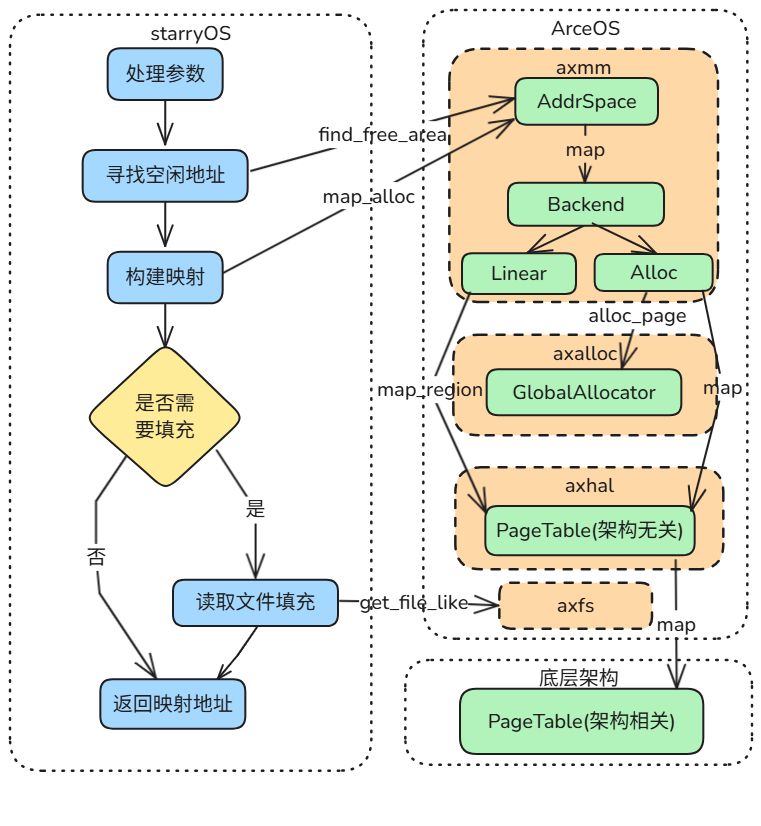
\includegraphics[width=0.7\linewidth, keepaspectratio]{syscall-mmap.png}
    \caption{mmap 系统调用流程}
    \label{fig:mmap}
\end{figure}


需要注意的是,由于 Lazy Map 机制的存在,不需要填充的内存区域不会立即被分配物理页,而是在第一次访问该内存区域并触发页面异常时才会分配物理页。该机制可能会导致内核在访问内存区域时出现 NotMapped 错误,因此需要在代码中调用 handle\_page\_fault 函数,为内存区域分配物理页,具体可以参考 AddrSpace 结构体的 clone\_or\_err 方法。

\begin{lstlisting}[language=c, caption=Lazy Map 机制下访问内存区域的处理]
let new_addr = match new_aspace.pt.query(vaddr) {
    Ok((paddr, _, _)) => paddr,
    // If the page is not mapped, try map it.
    Err(PagingError::NotMapped) => {
        if !backend.handle_page_fault(vaddr, area.flags(), &mut new\_aspace.pt) {
            return Err(AxError::NoMemory);
        }
        match new_aspace.pt.query(vaddr) {
            Ok((paddr, _, _)) => paddr,
            Err(_) => return Err(AxError::BadAddress),
        }
    }
    Err(_) => return Err(AxError::BadAddress),
};
\end{lstlisting}


除成功返回映射的起始地址外,starry-next 中 mmap 还有其他的返回情况:MAP\_FIXED 标志设置但地址为空,或者需要从文件读取数据填充映射区域但偏移量 offset 小于 0 或者超出文件大小,函数会返回 EINVAL 错误;若系统无法找到足够的连续空闲内存区域来完成映射操作,函数会返回 ENOMEM 错误;当需要从文件读取数据填充映射区域时,若文件描述符 fd 对应的文件对象无法转换为 arceos\_posix\_api::File 类型,函数会返回 EBADF 错误。

\subsection{munmap 系统调用}

munmap 用于解除进程地址空间中的内存映射。munmap 系统调用的原型如下:
\begin{lstlisting}[language=c, caption=munmap 系统调用函数原型]
int munmap(void addr[.length], size_t length);
\end{lstlisting}
munmap 系统调用共有 2 个参数,其中 addr 用于指定要解除映射的内存区域的起始地址,length 用于指定要解除映射的内存区域的长度。

munmap 系统调用的返回值是一个整数,通常为 0 表示成功,-1 表示失败。


如图\ref{fig:munmap},starry-next 中,munmap 系统调用的实现主要包括以下几个步骤:首先解析参数并检查其有效性;然后调用 AddrSpace 结构体的 unmap 方法,该方法会将指定的内存区域从页表中解除映射;刷新TLB;最后返回 0 表示成功。

\begin{figure}
    \centering
    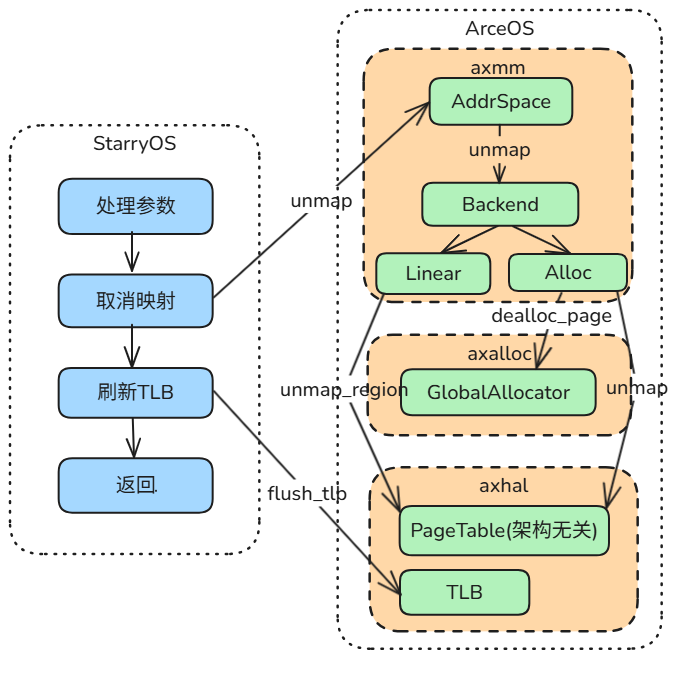
\includegraphics[width=0.7\linewidth, keepaspectratio]{syscall-unmap.png}
    \caption{munmap 系统调用流程}
    \label{fig:munmap}
\end{figure}


ArceOS 对 munmap 系统调用的支持方式与 mmap 系统调用类似,都是通过 AddrSpace 结构体向上提供接口,通过映射后端调用全局分配器和页表进行内存解除映射并释放物理页。 

另外,和 Linux 的标准实现相似,当需要取消映射的区域和当前存在的内存区域有重叠部分时,会将重叠部分的映射关系从页表中删除,并调整内存区域的起始地址和结束地址,如图\ref{fig:munmap2}所示,共存在三种情况:
\begin{enumerate}
    \item 完全覆盖:要解除映射的内存区域完全覆盖了当前存在的内存区域,此时需要将当前存在的内存区域从页表中删除,并将其从内存区域集合中移除。如图中第一项。
    \item 部分覆盖:要解除映射的内存区域位于当前存在的内存区域的中间部分,此时需要将当前存在的内存区域分为两部分,分别是要解除映射的内存区域的前半部分和后半部分,并加入到内存区域集合中,如图中第二项。
    \item 前后覆盖:要解除映射的内存区域包括当前存在的内存区域的左边界或右边界,需要调整当前存在的内存区域的起始地址或结束地址,如图中第三和第四项。
\end{enumerate}

\begin{figure}
    \centering
    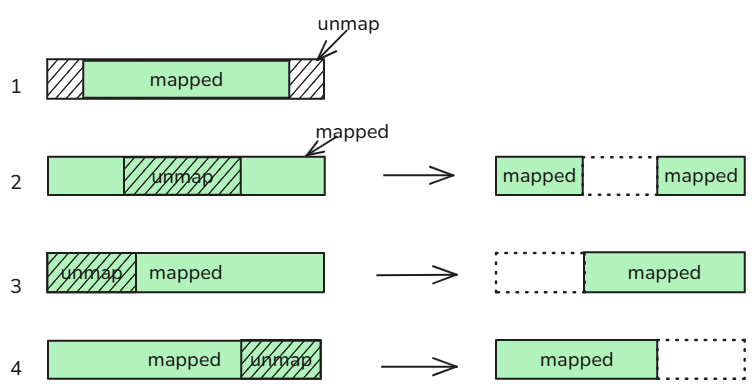
\includegraphics[width=0.7\linewidth, keepaspectratio]{syscall-munmap2.png}
    \caption{munmap 处理交叉区域}
    \label{fig:munmap2}
\end{figure}


\subsection{brk 系统调用}

brk 用于改变进程的堆顶位置。其原型如下:

\begin{lstlisting}[language=c, caption=brk 系统调用函数原型]
int brk(void addr);
\end{lstlisting}


可以看到,brk 系统调用只有一个参数,即 addr,用于指定数据段的结束位置。
其返回值是一个整数,通常为 0 表示成功,-1 表示失败。

starry-next 中,brk 系统调用通过设置任务信息结构体的 heap\_top 字段来改变堆顶地址。具体来说,brk 系统调用会将 heap\_top 字段设置为 addr,然后返回新的堆顶,但是如果 addr 小于当前 heap\_top,或者 addr 到堆底的距离大于进程的最大数据大小限制,那么 brk 系统调用会放弃设置新的堆顶并返回原来的堆顶地址。

需要注意的是,brk 系统调用只会改变进程的堆顶位置,并不会分配实际的物理内存。因此,在使用 brk 系统调用时,需要确保进程已经分配了足够的物理内存来支持新的堆顶位置。

\begin{figure}[H]
    \centering
    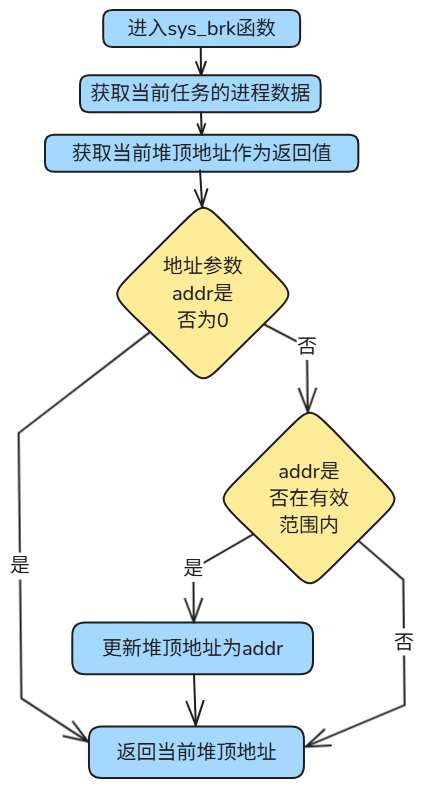
\includegraphics[width=0.4\linewidth, keepaspectratio]{syscall-brk-2.png}
    \caption{brk 系统调用流程}
    \label{fig:brk}
\end{figure}

\subsection{mprotect 系统调用}

mprotect 用于修改指定内存区域的保护属性。mprotect 系统调用的原型如下:
\begin{lstlisting}[language=c, caption=mprotect 系统调用函数原型]
int mprotect(void addr[.len], size_t len, int prot);
\end{lstlisting}

mprotect 系统调用接受三个参数:addr(要修改权限的内存区域的起始地址,必须是页面对齐的)、len(要修改权限的内存区域的长度)以及 prot(指定新的访问权限)。prot 参数可以是PROT\_NONE(无法访问)、PROT\_READ(可读取)、PROT\_WRITE(可写入)、PROT\_EXEC(可执行)、PROT\_GROWSDOWN(向下增长)、PROT\_GROWSUP(向上增长)的按位或组合。如果进程尝试以违反保护的方式访问内存,内核将生成一个 SIGSEGV 信号。

mprotect 系统调用的返回值是一个整数,通常为 0 表示成功,-1 表示失败。可能的错误包括:EFAULT——addr 指向的地址超出了进程的地址空间、EINVAL——len 为 0 或 prot 包含无效的标志、EACCES——进程没有足够的权限来修改内存区域的保护属性、ENOMEM——内存不足等。

如图\ref{fig:mprotect}所示,在进行地址长度页对齐等参数处理后,starry-next 使用了 AddrSpace 结构体的 protect 方法,进而通过 axhal 组件的页表接口来修改内存区域的保护属性。指定范围和当前存在的内存区域的关系和处理方式与 munmap 系统调用基本一致。但暂未实现 PROT\_GROWSDOWN 和 PROT\_GROWSUP 标志的处理。

\begin{figure}[H]
    \centering
    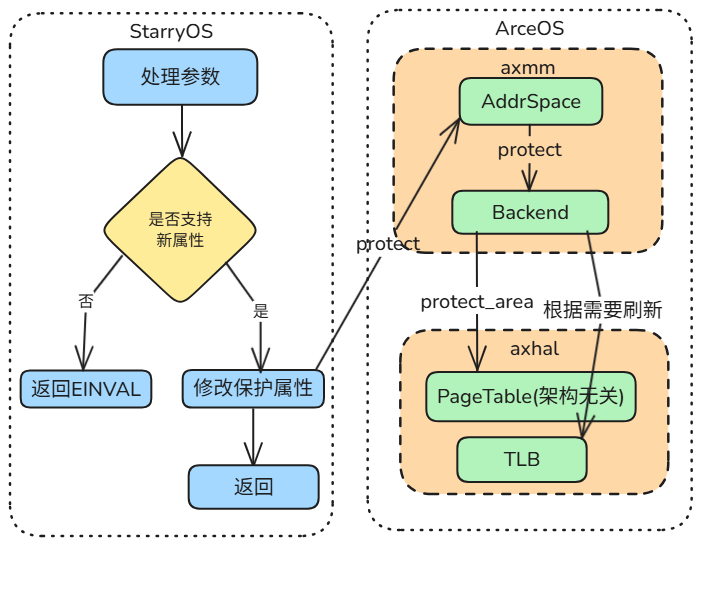
\includegraphics[width=1\linewidth, height = 8cm, keepaspectratio]{syscall-mprotect.png}
    \caption{mprotect 系统调用流程}
    \label{fig:mprotect}
\end{figure}

\section{内存管理子系统间接相关的系统调用}

\subsection{sysinfo 系统调用}

sysinfo 系统调用用于获取系统的信息,如内存使用情况、CPU 信息、文件系统信息等。sysinfo 系统调用的原型如下:
\begin{lstlisting}[language=c, caption=sysinfo 系统调用函数原型]
int sysinfo(struct sysinfo *info);
\end{lstlisting}
sysinfo 系统调用只有一个参数,即 info,用于存储系统信息的结构体指针。该结构体包含多个字段,例如 uptime(系统运行时间)、loads(1、5 和 15 分钟内的平均负载)、totalram 和 freeram(总内存和空闲内存)、sharedram 和 bufferram(共享内存和缓冲区内存)等。

% sysinfo 和内存管理的关系在于:sysinfo 系统调用可以获取系统的内存使用情况,包括总内存和空闲内存。因此在 ArceOS 的全局内存分配器的页分配器中,提供了接口以获取页分配器的总页数和空闲页数,这些信息可以用于计算总内存和空闲内存,并通过 sys\_sysconf 接口返回给 starry-next的 sysinfo 系统调用。

sysinfo 系统调用与包括内存管理在内的组件相关,例如通过 ArceOS 的 sys\_conf 接口获取 axconfig 组件中的核数等配置信息、axfs 组件的文件限制信息以及全局内存分配器的总页数和空闲页数;
通过 sys\_clock\_gettime 接口获取 axhal 组件的系统运行时间等。

\begin{figure}[H]
    \centering
    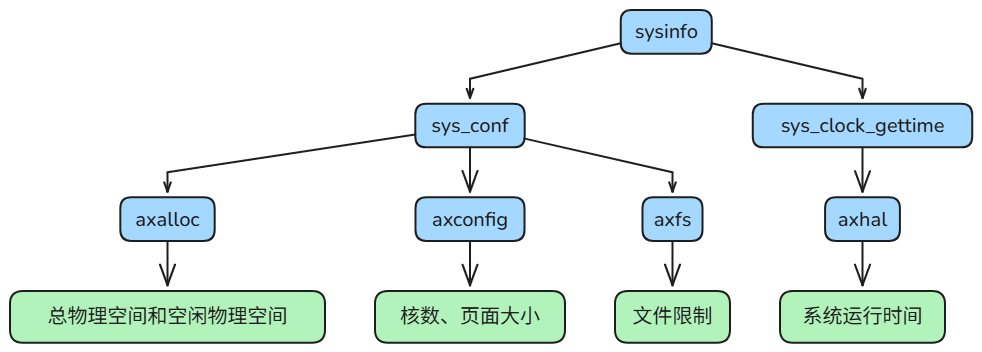
\includegraphics[width=1\linewidth, keepaspectratio]{syscall-sysinfo.png}
    \caption{sysinfo 系统调用流程}
    \label{fig:sysinfo-call}
\end{figure}

\subsection{arch\_prctl 系统调用}

arch\_prctl 系统调用用于设置或获取进程的特定架构相关的参数。其系统调用的原型如下:
\begin{lstlisting}[language=c, caption=arch\_prctl 系统调用函数原型]
int syscall(SYS_arch_prctl, int op, unsigned long addr);
int syscall(SYS_arch_prctl, int op, unsigned long *addr);
\end{lstlisting}

arch\_prctl 系统调用有两个参数,code 用于指定要设置或获取的参数,addr 用于指定参数的值,设置参数时会读取 addr 指向的内容,读取参数时将结果写入其指向的地址。常见的操作包括设置或获取进程的指针追踪(Pointer Tracing)状态、设置或获取 GS 段寄存器的值等。

arch\_prctl 系统调用的返回值是一个整数,通常为 0 表示成功,-1 表示失败。

当前 starry-next 中,arch\_prctl 系统调用支持四个参数的处理:GetFs、SetFs、GetGs 和 SetGs。其中 GetFs 和 SetFs 操作用于获取和设置进程的 FS 段寄存器的值,通过读取和设置 TrapFrame(陷阱帧)中的 TLS(Thread Local Storage,线程本地存储)寄存器实现;
GetGs 和 SetGs 操作用于读取和设置进程的内核 GS 段寄存器的值,通过读取和设置 x86 架构下 msr 寄存器实现。

\begin{figure}[H]
    \centering
    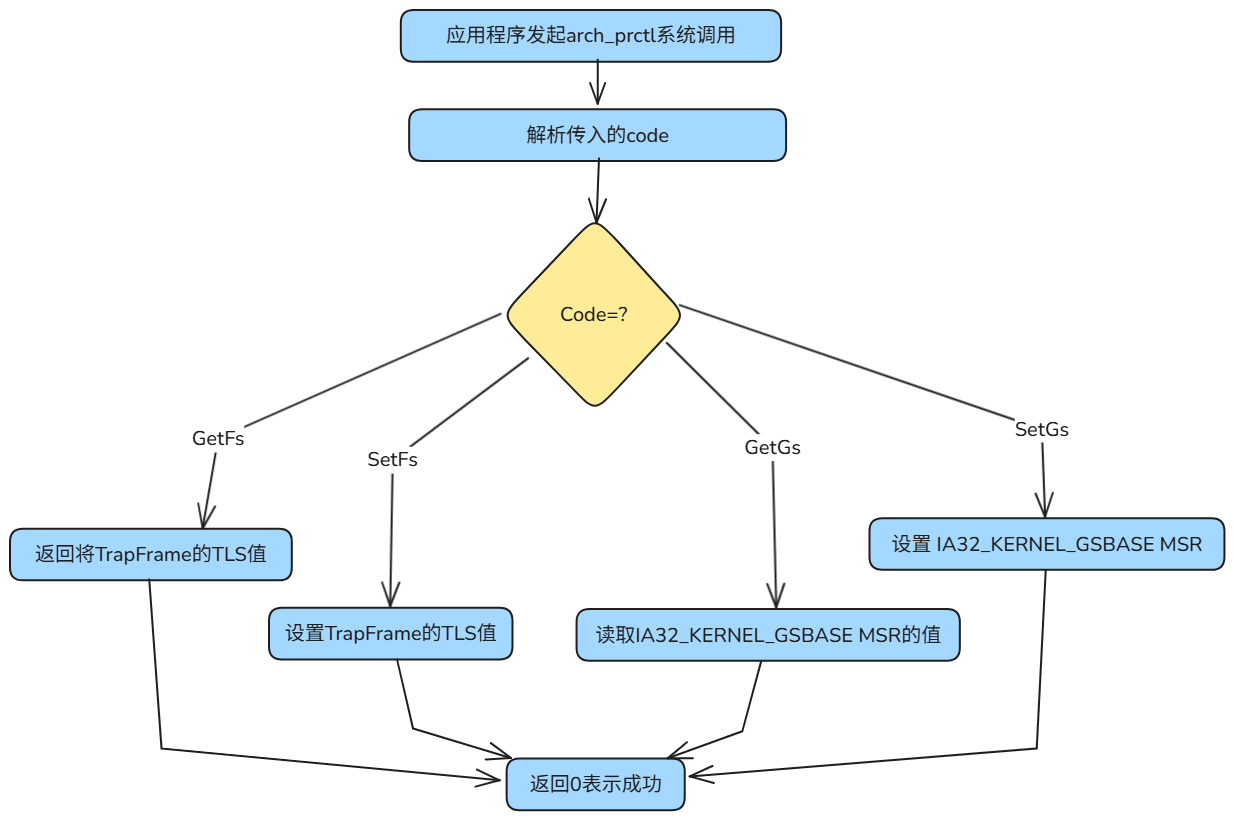
\includegraphics[width=1\linewidth, keepaspectratio]{syscall-arch-prctl-2.png}
    \caption{arch\_prctl 系统调用流程}
    \label{fig:arch-prctl}
\end{figure}

\subsection{prlimit64 系统调用}

prlimit64 系统调用用于设置或获取进程的资源限制,涉及操作系统的多个模块,例如栈大小和进程地址空间资源与内存管理模块有关,进程最大打开文件数与文件系统有关。prlimit64 系统调用的原型如下:
\begin{lstlisting}[language=c, caption=prlimit64 系统调用函数原型]
#include <sys/resource.h>
int prlimit64(pid_t pid, int resource, const struct rlimit64 *new_limit, struct rlimit64 *old_limit);
\end{lstlisting}

prlimit64 接受四个参数:pid——目标进程的进程ID,可以是当前进程或另一个进程)、
resource——要查询或设置的资源类型,例如 RLIMIT\_CORE(核心转储文件大小)、
RLIMIT\_CPU(CPU 时间)、RLIMIT\_DATA(数据段大小)等)、new\_limit——指向 rlimit64 结构体的指针,
用于指定新的资源限制,如果为 NULL 则表示仅获取当前限制,以及 old\_limit——指向 rlimit64 结构体的指针,
用于存储当前的资源限制,如果为 NULL 则不返回旧值。rlimit64 结构体包含 rlim\_cur(当前资源限制,又称软限制)和 rlim\_max(最大资源限制,
又称硬限制)两个字段,软限制是内核对相应资源强制执行的值,硬限制则作为软限制的上限。一个非特权进程只能将其软限制设置为从0到硬限制范围内的值,并且(不可逆地)降低其硬限制。

目前 starry-next 支持设置的资源限制包括 RLIMIT\_STACK(栈大小)和 RLIMIT\_NOFILE(最大打开文件数),二者分别通过修改进程信息结构体的 stack\_size 和 max\_files 字段来实现,其他类型的资源不会作处理。
同时限制了只有当前进程可以设置自己的资源限制,不能设置其他进程的资源限制,当传入的 pid 不为当前进程时,prlimit64 系统调用会返回 EINVAL 错误。

\begin{figure}[H]
    \centering
    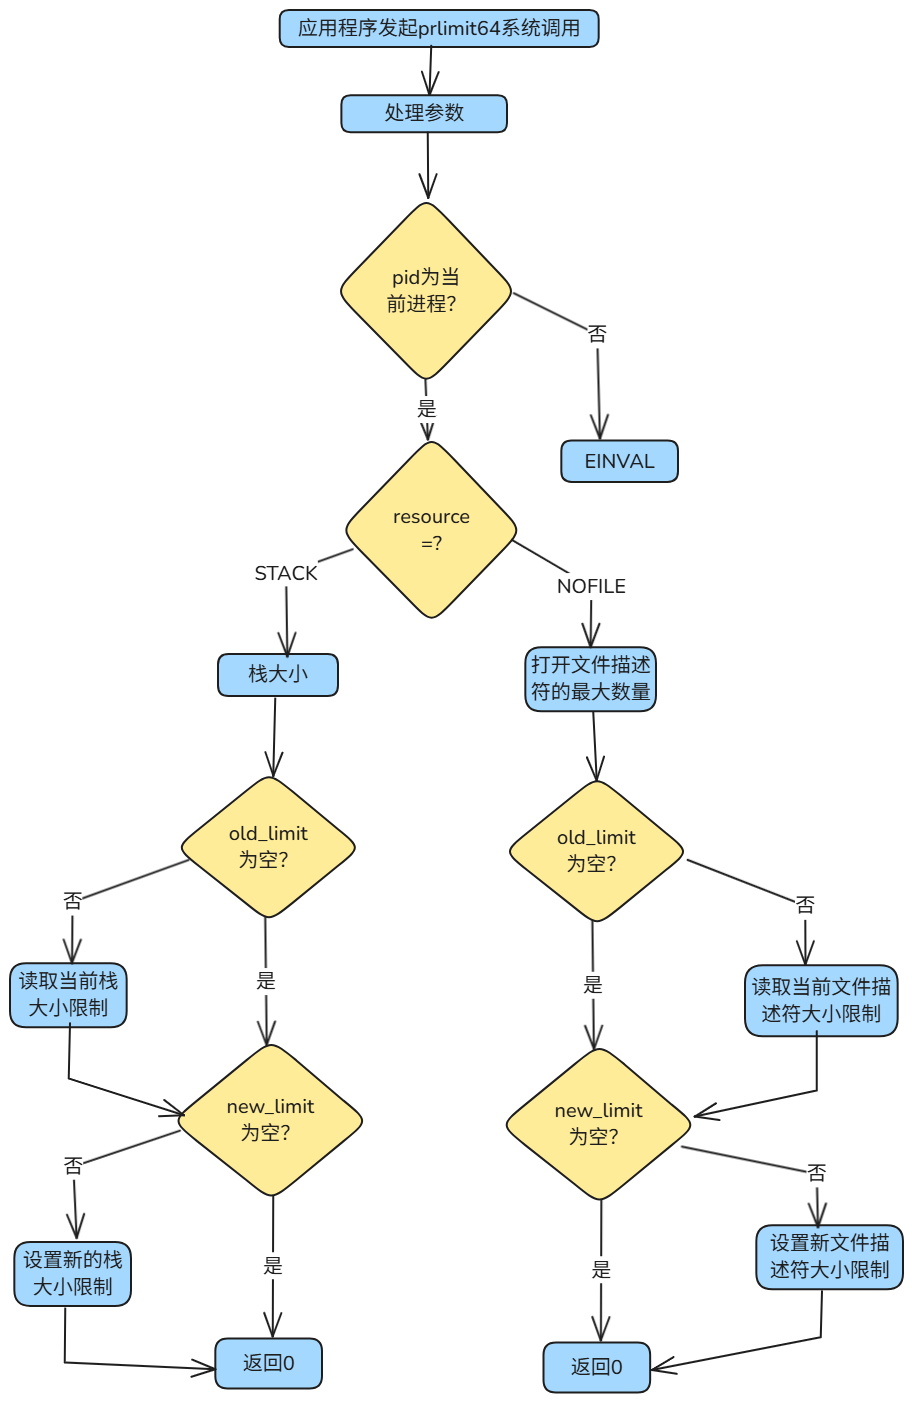
\includegraphics[width=0.7\linewidth, height=12.5cm]{syscall-prilimit64.png}
    \caption{prlimit64 系统调用流程}
    \label{fig:prlimit64}
\end{figure}

% !TeX root = ../cyh.tex

\chapter{实验环境与测试方法}

\section{实验环境}

% 本文采用 Linux 作为实验环境,使用 Ubuntu 20.04 作为主机操作系统,
为了验证 starry-next 内存管理模块及接口的设计与实现在 riscv64、x86\_64、loongarch64 和 aarch64 这四个架构下的正确性与性能,
我们使用了 qemu 模拟器来模拟这四个架构的运行环境,并且 qemu 模拟器的版本不应低于 8.2.0。qemu 是一个开源的虚拟机模拟器,支持多种硬件架构和操作系统,能够在主机上创建虚拟机并运行不同架构的操作系统。
同时,为了支持高版本的 qemu 模拟器,测例的本地运行都在 Ubuntu-24.04 下进行,并且需要在本地安装 rustling 工具链等 rust 相关工具,具体的操作可以参考项目的 README.md 文件。

另外,为了进行自动化测试,我们使用了 GitHub Actions 来实现自动化测试,定义了多个工作流配置文件,涵盖了不同架构和测试场景的自动化构建与验证。

测试分为功能测试和性能测试。

\section{功能测试}

\subsection{测试用例}

功能测试的测试用例分为两部分:开源测试用例和自定义测试用例。
其中开源测试用例主要来自 libc-test 库。libc-test 是一个针对 C 标准库(libc)功能及兼容性的检测工具。C 标准库作为 C 语言开发的基石,涵盖输入输出、内存管理、字符串操作等基础功能。
libc-test 借助一系列精心设计的测试用例,全面且细致地检验 C 标准库各功能模块,保障其在不同环境下的正确性和稳定性。在具体测试中,将编译完成的 libc-test 可执行文件作为输入,运行其中的静态与动态测试用例。
通过执行这些测试用例并检查输出结果,可判断待测内核是否能正确支持 C 标准库的各项功能,进而评估内核与 C 标准库的兼容性与稳定性。

尽管 libc-test 库提供了丰富的测试用例,可以涵盖大多数系统调用,例如 mmap、munmap、mprotect 等,但由于 libc-test 针对的是 C 标准库,而不是操作系统内核和系统调用的实现,
同时一部分系统调用无法使用 libc-test 进行测试,例如 sysinfo、prlimit64 等系统调用。
因此,我们还编写了一些自定义测试用例来验证 starry-next 内存管理模块的功能以及系统调用接口的正确性。这些用例将通过 C 标准库中 sys 子目录直接调用相关的系统调用,
并验证其返回值,例如:

\begin{lstlisting}[language=c, caption=prlimit64]
    #include <sys/syscall.h>
    syscall(SYS_prlimit64, getpid(), RLIMIT_STACK, NULL, &old_limit);
\end{lstlisting}

\begin{lstlisting}[language=c, caption=sysinfo]
    #include <sys/sysinfo.h>
    struct sysinfo info;
    sysinfo(&info);
\end{lstlisting}

在测例的编写和运行过程中,strace 指令可以帮助我们跟踪系统调用的执行情况,在 Ubuntu-24.04 下通过 strace 指令可以得到 x86\_64 架构下的系统调用信息,
使用 qemu 模拟器配合 strace 指令也可以得到其他架构下的系统调用信息。
这些不仅可以帮助验证测例的正确性,还可以作为对照组可以帮助我们分析 starry-next 内存管理模块的实现是否符合 Linux 的标准实现,
以及系统调用的实现的正确性,从而进行进一步的调试和优化。

\subsection{测试结果与分析}

接下来,我们将从系统调用的角度对测试结果进行展示与分析。

\subsubsection{mmap 和 munmap 系统调用}

要验证 mmap 系统调用的正确性,一方面可以通过本地使用 strace 指令在 libc-test 中找出使用了该系统调用的测试用例,例如 fdopen,这里我们展示 fdopen 测例在 x86\_64 架构下的测试结果:
\begin{lstlisting}[language=bash, caption=fdopen 测试结果]
    ========== START entry-static.exe fdopen ==========
    ...
    [  1.836930 1:11 starry::syscall:12] Syscall mmap
    [  1.838002 1:11 starry_api::imp::mm::mmap:100] mmap: addr: 0x0, length: 1000, prot: MmapProt(PROT_READ | PROT_WRITE), flags: MmapFlags(MAP_PRIVATE | MAP_ANONYMOUS), fd0
    [  1.845482 1:11 starry::syscall:145] Syscall mmap return 4096
    ...
    [  2.024200 1:11 starry::syscall:12] Syscall munmap
    [  2.027765 1:11 starry::syscall:145] Syscall munmap return 0
    ...
    Pass!
    ========== END entry-static.exe fdopen ==========
\end{lstlisting}

从结果中可以看到,fdopen 测试用例执行了 mmap 系统调用,创建一个长度为 1000 字节的匿名私有映射,这段内存区域可以被读取和写入。返回值为 4096,说明系统自动选择的起始地址是 0x1000,映射成功。
并且测例整体也是通过的,说明 mmap 系统调用匿名映射部分的实现是正确的。而 munmap 系统调用的返回值为 0,说明解除映射成功。

另一方面,我们还可以通过自定义测试用例来验证 mmap 系统调用的正确性,例如:
\begin{lstlisting}[language=c, caption=自定义 mmap 测试用例]
    fd = open("test_mmap.txt", O_RDWR | O_CREATE);
    array = mmap(NULL, kst.st_size, PROT_WRITE | PROT_READ, MAP_FILE | MAP_SHARED, fd, 0);
    printf("mmap content: %s\n", array);
\end{lstlisting}

在这个测试用例中,我们打开了一个文件,并使用 mmap 系统调用将该文件映射到内存中,然后读取文件内容并打印出来。
从运行结果来看,内核成功地将文件映射到内存中,并且可以正确读取文件内容,说明 mmap 系统调用的实现是正确的。

\begin{lstlisting}[language=bash, caption=自定义 mmap 测试用例结果]
========== START test_mmap ==========
file len: 27
mmap content:   Hello, mmap successfully!
========== END test_mmap ==========
\end{lstlisting}

\subsubsection{brk 系统调用}

brk 系统调用用于设置进程的堆空间的结束地址,因而要验证 brk 系统调用的正确性,可以通过反复设置和获取堆空间的结束地址来验证其实现是否正确。
例如 libc-test 中的 mbc 测试用例,在 x86\_64 架构下的测试结果如下: 
\begin{lstlisting}[language=c, caption=brk]
    [  1.817163 1:11 starry::syscall:12] Syscall brk
    [  1.819303 1:11 starry::syscall:145] Syscall brk return 1073741824
    [  1.821880 1:11 starry::syscall:12] Syscall brk
    [  1.823235 1:11 starry::syscall:145] Syscall brk return 1073750016
\end{lstlisting}

从结果中可以看到,brk 系统调用的返回值是 1073741824 和 1073750016,分别表示堆空间的结束地址是 1GB 和 1.5GB。
这说明 brk 系统调用的实现是正确的。

\subsubsection{sysinfo 和 prlimit64 系统调用}

sysinfo 和 prlimit64 系统调用的自定义测试用例主要是通过获取系统信息和进程限制来验证其实现是否正确。在 riscv64 架构下的测试结果如下:

\begin{figure}
    \centering
    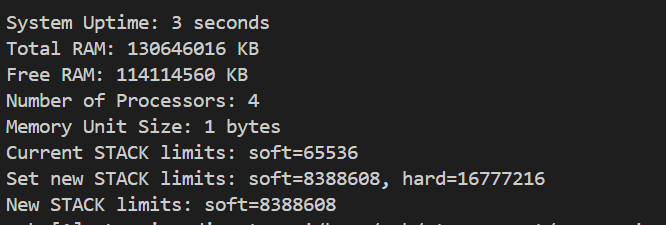
\includegraphics[width=0.5\linewidth]{sysinfo.png}
    \caption{sysinfo 和 prlimit64 测试结果}
    \label{fig:sysinfo-test}
\end{figure}

从图\ref{fig:sysinfo-test}中可以看到,sysinfo 系统调用返回了系统的内存使用情况,包括总内存和空闲内存等信息,并且 prlimit64 系统调用返回了进程用户栈的限制信息。
同时,当设置用户栈大小时,prlimit64 系统调用正确使用了新的软限制值,
这说明 sysinfo 和 prlimit64 系统调用用户栈选项的功能正常。而 prlimit64 的最大文件数量限制则可以通过 libc-test 的 rlimit\_open\_files 测试用例来验证,
该测例会在设置资源限制后重复创建新的文件描述符(打开文件)至失败,并取当前最大文件描述符和资源限制值进行比较,相等则说明实现正确。该测例也是通过的。

\begin{figure}
    \centering
    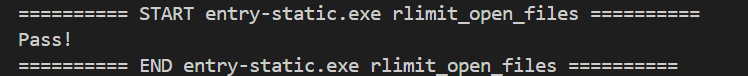
\includegraphics[width=0.5\linewidth]{prlimit64.png}
    \caption{rlimit\_open\_files 测例结果}
    \label{fig:prlimit64-test}
\end{figure}

\section{性能测试}

当前并未对 starry-next 内存管理模块的性能进行专项测试,
但在功能测试中,部分测例的运行时间也可以作为性能测试的参考。我们将 starry-next 内存管理模块的性能与 Linux 的标准实现进行对比,
以验证 starry-next 内存管理模块的性能是否符合 Linux 的标准实现。

以功能测试中的自定义 mmap 测试用例为例,
在 x86\_64 架构下的测试结果如下:
\begin{figure}[H]
    \centering  % 图片全局居中
    \begin{subfigure}[t]{0.45\textwidth}
        \centering
        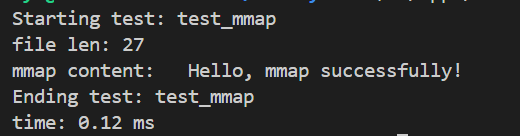
\includegraphics[width=\linewidth]{s2-local.png}
        \caption{Linux}
        \label{fig:sub.1}
    \end{subfigure}
    \hfill % 添加一些水平间距
    \begin{subfigure}[t]{0.45\textwidth}
        \centering
        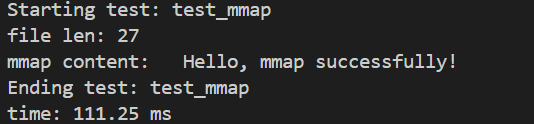
\includegraphics[width=\linewidth]{s2-starry.png}
        \caption{starry-next}
        \label{fig:sub.2}
    \end{subfigure}
    \caption{自定义 mmap 测试用例的运行时间对比}
    \label{Fig.main}
\end{figure}

不难看出,starry-next 花费的时间远高于本机的运行时间。为了减少其他模块的影响,
本文还设计了一个简单的 c 程序,该程序重复进行系统调用,
并将其运行时间与 Linux 的标准实现进行对比,
结果如下:

\begin{figure}[H]
    \centering  % 图片全局居中
    \begin{subfigure}[t]{0.45\textwidth}
        \centering
        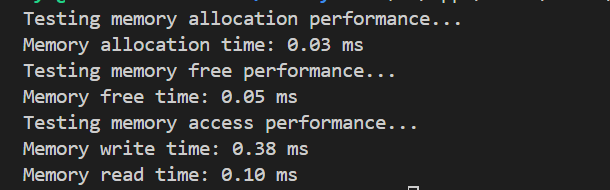
\includegraphics[width=\linewidth]{s1.png}
        \caption{Linux}
        \label{fig:sub.3}
    \end{subfigure}
    \hfill % 添加一些水平间距
    \begin{subfigure}[t]{0.45\textwidth}
        \centering
        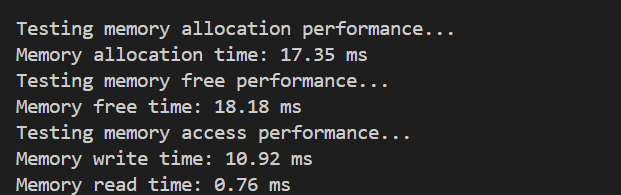
\includegraphics[width=\linewidth]{s1-starry.png}
        \caption{starry-next}
        \label{fig:sub.4}
    \end{subfigure}
    \caption{重复进行系统调用的运行时间对比}
    \label{Fig.main2}
\end{figure}

由图\ref{Fig.main2}可见starry-next 在映射、解除映射、读取和写入数据等方面花费的时间远高于本机的运行时间,
尽管 starry-next 的运行还要受到 qemu 模拟器的影响,自身也实现了 Lazy Map 等内存管理方面的优化机制,
但总体来说,其性能仍有很大的提升空间。
% !TeX root = ../cyh.tex

\chapter{结论与展望}

\section{结论}

到目前为止,我们已经基本完成了 starry-next 内存管理模块及其接口的设计与实现,并且对其进行了测试。我们的实现与 Linux 内核的内存管理模块接口基本一致,并且在功能测试中表现良好,
性能方面则需要进一步测试和优化。
具体的代码已开源至 \href{https://github.com/chenyihu21/starry-next}{GitHub}。

在开发过程中,由于操作系统的各模块间存在一定的依赖关系,
我们使用了多种协同开发 OS 的方法,包括使用 GitHub 的 issue 和 pull request 进行协作,
根据模块和系统调用分配任务,以通过某个测例为目的进行调试等。
我们不仅参与了宏内核接口的设计、实现与测试,还一定程度上参与了基座微内核 ArceOS 的修改。
另外,我们还将开发过程中的问题和解决方法记录在了实验报告中,以便后续的开发工作中可以参考。
希望这些工作能为后续组件化操作系统的开发提供一些参考和帮助。

\section{展望}

在未来的工作中,我们计划进一步完善 starry-next 内存管理模块及其接口,
包括完善当前仅实现部分功能的系统调用接口、优化内存管理模块的性能等方面。另外,当前 starry-next 内存管理模块还未支持各类页面置换算法,
我们计划在未来的工作中增加对不同页面置换算法的支持,以提高内存管理模块的性能和效率。
同时,增加对内存管理模块的安全性和稳定性的支持也会纳入未来的计划,
以确保内存管理模块在实际应用中能够稳定运行。

% 参考文献
\bibliography{ref/refs}  % 参考文献使用 BibTeX 编译
% \printbibliography       % 参考文献使用 BibLaTeX 编译

% 附录
\appendix
% % !TeX root = ../cyh.tex

\begin{survey}
\label{cha:survey}

\title{Title of the Survey}
\maketitle


\tableofcontents


本科生的外文资料调研阅读报告。


\section{Figures and Tables}

\subsection{Figures}

An example figure in appendix (Figure~\ref{fig:appendix-survey-figure}).

\begin{figure}
  \centering
  
\includegraphics[width=0.6\linewidth]{example-image-a.pdf}
  \caption{Example figure in appendix}
  \label{fig:appendix-survey-figure}
\end{figure}


\subsection{Tables}

An example table in appendix (Table~\ref{tab:appendix-survey-table}).

\begin{table}
  \centering
  \caption{Example table in appendix}
  \begin{tabular}{ll}
    \toprule
    File name       & Description                                         \\
    \midrule
    thuthesis.dtx   & The source file including documentation and comments \\
    thuthesis.cls   & The template file                                   \\
    thuthesis-*.bst & BibTeX styles                                       \\
    thuthesis-*.bbx & BibLaTeX styles for bibliographies                  \\
    thuthesis-*.cbx & BibLaTeX styles for citations                       \\
    \bottomrule
  \end{tabular}
  \label{tab:appendix-survey-table}
\end{table}


\section{Equations}

An example equation in appendix (Equation~\eqref{eq:appendix-survey-equation}).
\begin{equation}
  \frac{1}{2 \uppi \symup{i}} \int_\gamma f = \sum_{k=1}^m n(\gamma; a_k) \mathscr{R}(f; a_k)
  \label{eq:appendix-survey-equation}
\end{equation}


\section{Citations}

Example\cite{dupont1974bone} citations\cite{merkt1995rotational} in appendix
\cite{dupont1974bone,merkt1995rotational}.


% 默认使用正文的参考文献样式;
% 如果使用 BibTeX,可以切换为其他兼容 natbib 的 BibTeX 样式。
\bibliographystyle{unsrtnat}
% \bibliographystyle{IEEEtranN}

% 默认使用正文的参考文献 .bib 数据库;
% 如果使用 BibTeX,可以改为指定数据库,如 \bibliography{ref/refs}。
\printbibliography

\end{survey}
       % 本科生:外文资料的调研阅读报告
% % !TeX root = ../cyh.tex

\begin{translation}
\label{cha:translation}

\title{书面翻译题目}
\maketitle

\tableofcontents


本科生的外文资料书面翻译。


\section{图表示例}

\subsection{图}

附录中的图片示例(图~\ref{fig:appendix-translation-figure})。

\begin{figure}
  \centering
  
\includegraphics[width=0.6\linewidth]{example-image-a.pdf}
  \caption{附录中的图片示例}
  \label{fig:appendix-translation-figure}
\end{figure}


\subsection{表格}

附录中的表格示例(表~\ref{tab:appendix-translation-table})。

\begin{table}
  \centering
  \caption{附录中的表格示例}
  \begin{tabular}{ll}
    \toprule
    文件名          & 描述                         \\
    \midrule
    thuthesis.dtx   & 模板的源文件,包括文档和注释 \\
    thuthesis.cls   & 模板文件                     \\
    thuthesis-*.bst & BibTeX 参考文献表样式文件    \\
    thuthesis-*.bbx & BibLaTeX 参考文献表样式文件  \\
    thuthesis-*.cbx & BibLaTeX 引用样式文件        \\
    \bottomrule
  \end{tabular}
  \label{tab:appendix-translation-table}
\end{table}


\section{数学公式}

附录中的数学公式示例(公式\eqref{eq:appendix-translation-equation})。
\begin{equation}
  \frac{1}{2 \uppi \symup{i}} \int_\gamma f = \sum_{k=1}^m n(\gamma; a_k) \mathscr{R}(f; a_k)
  \label{eq:appendix-translation-equation}
\end{equation}


\section{文献引用}

附录\cite{dupont1974bone}中的参考文献引用\cite{merkt1995rotational}示例
\cite{dupont1974bone,merkt1995rotational}。


\appendix

\section{附录}

附录的内容。


% 书面翻译的参考文献
% 默认使用正文的参考文献样式;
% 如果使用 BibTeX,可以切换为其他兼容 natbib 的 BibTeX 样式。
\bibliographystyle{unsrtnat}
% \bibliographystyle{IEEEtranN}

% 默认使用正文的参考文献 .bib 数据库;
% 如果使用 BibTeX,可以改为指定数据库,如 \bibliography{ref/refs}。
\printbibliography

% 书面翻译对应的原文索引
\begin{translation-index}
  \nocite{mellinger1996laser}
  \nocite{bixon1996dynamics}
  \nocite{carlson1981two}
  \bibliographystyle{unsrtnat}
  \printbibliography
\end{translation-index}

\end{translation}
  % 本科生:外文资料的书面翻译
% % !TeX root = ../cyh.tex

\chapter{补充内容}

附录是与论文内容密切相关、但编入正文又影响整篇论文编排的条理和逻辑性的资料,例如某些重要的数据表格、计算程序、统计表等,是论文主体的补充内容,可根据需要设置。

附录中的图、表、数学表达式、参考文献等另行编序号,与正文分开,一律用阿拉伯数字编码,
但在数码前冠以附录的序号,例如“图~\ref{fig:appendix-figure}”,
“表~\ref{tab:appendix-table}”,“式\eqref{eq:appendix-equation}”等。


\section{插图}

% 附录中的插图示例(图~\ref{fig:appendix-figure})。

\begin{figure}
  \centering
  
\includegraphics[width=0.6\linewidth]{example-image-a.pdf}
  \caption{附录中的图片示例}
  \label{fig:appendix-figure}
\end{figure}


\section{表格}

% 附录中的表格示例(表~\ref{tab:appendix-table})。

\begin{table}
  \centering
  \caption{附录中的表格示例}
  \begin{tabular}{ll}
    \toprule
    文件名          & 描述                         \\
    \midrule
    thuthesis.dtx   & 模板的源文件,包括文档和注释 \\
    thuthesis.cls   & 模板文件                     \\
    thuthesis-*.bst & BibTeX 参考文献表样式文件    \\
    thuthesis-*.bbx & BibLaTeX 参考文献表样式文件  \\
    thuthesis-*.cbx & BibLaTeX 引用样式文件        \\
    \bottomrule
  \end{tabular}
  \label{tab:appendix-table}
\end{table}


\section{数学表达式}

% 附录中的数学表达式示例(式\eqref{eq:appendix-equation})。
\begin{equation}
  \frac{1}{2 \uppi \symup{i}} \int_\gamma f = \sum_{k=1}^m n(\gamma; a_k) \mathscr{R}(f; a_k)
  \label{eq:appendix-equation}
\end{equation}


\section{文献引用}

附录\cite{dupont1974bone}中的参考文献引用\cite{zhengkaiqing1987}示例
\cite{dupont1974bone,zhengkaiqing1987}。

\printbibliography


% 其他部分
\backmatter

% 致谢
% % !TeX root = ../cyh.tex

\begin{acknowledgements}
  衷心感谢导师×××教授和物理系××副教授对本人的精心指导。他们的言传身教将使我终生受益。

  在美国麻省理工学院化学系进行九个月的合作研究期间,承蒙 Robert Field 教授热心指导与帮助,不胜感激。

  感谢×××××实验室主任×××教授,以及实验室全体老师和同窗们学的热情帮助和支持!

  本课题承蒙国家自然科学基金资助,特此致谢。
\end{acknowledgements}


% 声明
% 各类开题报告通常不需要
% \statement[page-style=empty]  % 编译生成的声明页默认不含页眉页脚,以避免页码变化带来问题
% 在提交终稿时,插入签字后的扫描件 scan-statement.pdf,并添加页眉页脚
% \statement[page-style=plain, file=scan-statement.pdf]
% 如确实需要在电子版中直接页眉页脚,则使用
% \statement[page-style=plain]

% 个人简历、在学期间完成的相关学术成果
% 本科生可以附个人简历,也可以不附个人简历
% % !TeX root = ../cyh.tex

\begin{resume}

  \section*{个人简历}

  197× 年 ×× 月 ×× 日出生于四川××县。

  1992 年 9 月考入××大学化学系××化学专业,1996 年 7 月本科毕业并获得理学学士学位。

  1996 年 9 月免试进入清华大学化学系攻读××化学博士至今。


  \section*{在学期间完成的相关学术成果}

  \subsection*{学术论文}

  \begin{achievements}
    \item Yang Y, Ren T L, Zhang L T, et al. Miniature microphone with silicon-based ferroelectric thin films[J]. Integrated Ferroelectrics, 2003, 52:229-235.
    \item 杨轶, 张宁欣, 任天令, 等. 硅基铁电微声学器件中薄膜残余应力的研究[J]. 中国机械工程, 2005, 16(14):1289-1291.
    \item 杨轶, 张宁欣, 任天令, 等. 集成铁电器件中的关键工艺研究[J]. 仪器仪表学报, 2003, 24(S4):192-193.
    \item Yang Y, Ren T L, Zhu Y P, et al. PMUTs for handwriting recognition. In press[J]. (已被Integrated Ferroelectrics录用)
  \end{achievements}


  \subsection*{专利}

  \begin{achievements}
    \item 任天令, 杨轶, 朱一平, 等. 硅基铁电微声学传感器畴极化区域控制和电极连接的方法: 中国, CN1602118A[P]. 2005-03-30.
    \item Ren T L, Yang Y, Zhu Y P, et al. Piezoelectric micro acoustic sensor based on ferroelectric materials: USA, No.11/215, 102[P]. (美国发明专利申请号.)
  \end{achievements}

\end{resume}



% 本科生格式:

% \begin{resume}
%   \section*{学术论文}
%
%   \begin{achievements}
%     \item ZHOU R, HU C, OU T, et al. Intelligent GRU-RIC Position-Loop
%       Feedforward Compensation Control Method with Application to an
%       Ultraprecision Motion Stage[J], IEEE Transactions on Industrial
%       Informatics, 2024, 20(4): 5609-5621.
%
%     \item 杨轶, 张宁欣, 任天令, 等. 硅基铁电微声学器件中薄膜残余应力的研究[J].
%       中国机械工程, 2005, 16(14):1289-1291.
%
%     \item YANG Y, REN T L, ZHU Y P, et al. PMUTs for handwriting recognition.
%       In press[J]. (已被Integrated Ferroelectrics录用)
%
%   \end{achievements}
%
%
%   \section*{专利}
%
%   \begin{achievements}
%     \item 胡楚雄, 付宏, 朱煜, 等. 一种磁悬浮平面电机: ZL202011322520.6[P]. 2022-04-01.
%
%     \item REN T L, YANG Y, ZHU Y P, et al. Piezoelectric micro acoustic sensor
%       based on ferroelectric materials: No.11/215, 102[P]. (美国发明专利申请号.)
%
%   \end{achievements}
% \end{resume}


% 指导教师/指导小组评语
% 本科生不需要
% % !TeX root = ../cyh.tex

\begin{comments}
% \begin{comments}[name = {指导小组评语}]
% \begin{comments}[name = {Comments from Thesis Supervisor}]
% \begin{comments}[name = {Comments from Thesis Supervision Committee}]

  论文提出了……

\end{comments}


% 答辩委员会决议书
% 本科生不需要
% % !TeX root = ../cyh.tex

\begin{resolution}

  论文提出了……

  论文取得的主要创新性成果包括:

  1. ……

  2. ……

  3. ……

  论文工作表明作者在×××××具有×××××知识,具有××××能力,论文××××,答辩××××。

  答辩委员会表决,(×票/一致)同意通过论文答辩,并建议授予×××(姓名)×××(门类)学博士/硕士学位。

\end{resolution}


% 本科生的综合论文训练记录表(扫描版)
% \record{file=scan-record.pdf}

\end{document}
